\documentclass[11pt]{article}

\usepackage[a4paper, margin=1in]{geometry}
\usepackage[british]{babel}
\usepackage[backend=biber, style=numeric-comp]{biblatex}
\usepackage{amssymb}
\usepackage{amsmath}
\usepackage{listings, listings-rust}
\usepackage{tikz-cd}
\usepackage{graphicx}

\addbibresource{bibliography.bib}

\graphicspath{./}

\title{Lambda Calculus and its Implications in Computer Science}
\author{Joris Klaasse Bos\\ Zaanlands Lyceum}

\begin{document}

\maketitle
\newpage

\section*{Preface}
\addcontentsline{toc}{section}{Preface}

% todo: Something about PWS

The reason I chose to write about this subject, is that it combines two things
I enjoy: abstract mathematics and computer science. I have been programming for
about five to six years now. I mainly enjoy low-level programming,
so---naturally---C is my most used language and I am most familiar with a
simple procedural paradigm. Such a paradigm is, however, not always very easy
to use when working with very large and complex systems. I, as many, started
out with object-oriented programming (OOP), but I did not like that very much.
Therefore, I have been exploring alternative paradigms, including data-oriented
programming and functional programming. I am quite familiar with data-oriented
programming and the Rust programming language by now, but functional
programming isn't something I've ever really got into yet. I did find out about
lambda calculus and combinatory logic, which intrigued me, but I haven’t got
into it beyond a basic level of understanding. That is why I decided to
research it for this work. 

I have some things to note on the structure and style of this work. Firstly,
the structure. The work starts with some introductory information about lambda
calculus and its history. It goes on to explain the simple syntax of lambda
calculus and how it can be used. The next section goes into lambda calculus
in-depth. It really shows how lambda calculus is used as a Turing complete
mathematical system. The section after that explains functional programming. It
shows how lambda calculus can be turned into a programming language, and
explains why it is useful by comparing it to other paradigms, namely procedural
imperative programming (what that means isn't really of importance right now).
The final few sections are smaller; they really just meant to illustrate what
is said in the preceding sections.

Secondly, every reference will be denoted with a number in braces which
corresponds with a work found in the back on the references page. Many of my
sources, however, aren't on there, because I didn't directly refer to them.
Those sources will be displayed on the page after the references, the
bibliography (as of now, I haven't yet compiled those sources and created that
page).

As for the style in which I explain lambda calculus, I may differ in it from
how other literature usually approaches the topic. Lambda calculus is often
used in a mathematical context, so people often write in a very mathematical
style. People don't usually write pure lambda calculus, they borrow a lot of
symbols from other mathematical disciplines, such as logic. Nor do people
define it in words, but also with mathematical symbols and definitions. I try
to keep the use of these symbols to a minimum so as to lower the barrier to
entry. Rather than using mathematical symbols and definitions, I use my words
to explain the lambda calculus, thus this work is written in a more prose-like
style, rather than a strictly mathematical one. I think that lambda calculus is
simple enough that, when explained well, most people should be able to follow
it. On a similar note, I think that the way this work is written, most people
who are not familiar with mathematical literature should be able to follow it.

\newpage

\tableofcontents
\newpage

\section{Introduction}

With the decline of OOP (object-oriented programming), many other paradigms are
gaining in popularity. One increasingly popular paradigm is functional
programming. Functional programming is fundamentally based on lambda calculus
and it has been seeping into other paradigms and into mainstream languages.
Most of the popular languages now implement lambda functions and have ways to
write in a more declarative style of programming. In this work I will look at
all the ways lambda calculus has influenced computer science and how it may do
so in the future.

\section{Introduction to lambda calculus}

Lambda calculus is, as its name suggests, a calculus. A calculus is a system of
manipulating symbols, which by themselves don't have any meaning, in a way that
is somehow meaningful. We all know algebra. Algebra itself doesn't have an
innate meaning, but we can use it to represent and solve real world problems.
Algebra, however, is limited. Not every problem can be represented in algebra.
There are many branches of mathematics that use different systems. One example
would be formal logic, which is used for logical operations on booleans.
Another such example is lambda calculus.

\subsection{A short history\label{history}}

People always trusted mathematics to be true and relied on it heavily. If
something was proven true with mathematical logic, then that must be true.
However, starting from the late 19th century, people ran into paradoxes. People
made a distinction between reasoning that is rigorous and reasoning that
isn't---reasoning that is logical, and reasoning that is psychological. The
fact that mathematical logic, which people looked at for rigorousness, is
infested with paradoxes and self-reference was very troubling for people at the
time.

The concept of mathematics and mathematical logic wasn't well defined, so
people started to think about the formalisation of mathematical logic to try to
solve these issues. People wanted a system that would encapsulate all of
mathematical logic. Preferably this system would be simple, clean and
intuitive.

Throughout the late 19th and early 20th centuries, people started formally
defining and redefining different aspects of mathematics. \textcite{frege1879}
wrote about propositional calculus and functions as graphs, and in doing so
re-evaluated the concept of functions and was already using concepts like
Currying functions (more on this in section \ref{syntax}) without really giving
thought to it. \textcite{peano1889} invented the Peano axioms and Peano
arithmetic as a way of defining natural numbers. He was not the first to
attempt defining natural numbers, but he was the most successful.
\textcite{schonfinkel1924} invented combinatory logic, which was later
rediscovered and improved on by \textcite{curry1930}, as a way to remove the
need for quantified variables in logic.

One major attempt to define all of mathematics was done by
\textcite{russell1997}. They wrote a book that would become well know in all of
mathematics and logic. This book is called \emph{Principia Mathematica}. They
did, however, run into a few problems, which arose from self-reference. To
solve these problems that this paradoxical self-reference brought with it, they
invented an elaborate system, the theory of types, to circumvent/eliminate it.
It was a very carefully crafted bastion against self-reference ever coming up
in their system, which was not very simple, clean or intuitive.

People praised \emph{PM} as they thought they had finally done it; they had
formalised all of mathematical logic, they had realised the dream of grounding
all of mathematics in logic. But in Vienna, Gödel was sceptical of this book.
He started seeing some cracks, he felt that there was something wrong about
this attempt. Gödel felt that self-reference was a fundamental part of
mathematical logic. Then he went out and actually proved that there is no
consistent system of axioms whose theorems can be listed by an effective
procedure that is capable of proving all truths about arithmetic of natural
numbers\footnote{This is a definition of the first incompleteness theorem I got
from \textcite{wiki:Incompleteness_theorems}} \parencite{godel1931}, meaning
that such a system is either inconsistent or incomplete\footnote{Incompleteness
means that there are things that are true, but are not provable.}, greatly
disturbing many mathematicians and upending mathematics as they knew it.

During this time, in this environment of the formalisation of mathematical
logic, \textcite{church1932} invented the lambda calculus. Lambda calculus is a
very simple and minimalistic system of substitution. A little while later,
\textcite{turing1936, turing1937correction} invented Turing machines. Turing
machines are conceptual mathematical machines that function based on
state---they were state machines. These could perform all kinds of mathematical
and logical computations. He was not the first to invent computers, but he was
the first to work them out as well as he did (and, as you probably know, he
built one which he cracked the German enigma code with).

There was this problem that has a few different names. It is often known as the
\emph{halting problem} or the \emph{Entscheidungsproblem}, which is German for
\emph{decision problem}. The halting problem and decision problem aren't
exactly synonyms, but they come down to the same thing. Basically, it asks
whether it is possible to know via an algorithm whether a computation will
complete execution or result in an infinite loop. In 1936,
\textcite{turing1936, turing1937correction} spent a long time proving, using
his Turing machines, that this isn't possible, but it didn't get published
until early 1937. Also in 1936, \textcite{church1936} proved the same thing
using lambda calculus and happened to publish it before Turing did. When Turing
finally got around to publishing his proof, he found out that he was beaten to
it by Church. He wasn't too pleased. What is interesting, though, is that
lambda calculus and Turing machines take two completely different approaches.
Turing machines function entirely on state, while lambda calculus is completely
stateless (we'll look at this later). Turing thought this was interesting too,
so he researched lambda calculus and how it relates to his Turing machines, and
proved that they are formally equivalent \parencite{turing1937computability}. 

Why do I tell you all this? Well, your main takeaway should be that even though
lambda calculus is a very simple system, which at first glance might not seem
to be very semantic or seem to have any real world implications, it actually is
Turing complete. Lambda calculus and Turing machines take wildly different
approaches: one state based, the other stateless. Another difference is that
Turing machines can be physically built. We can, however, use lambda calculus
on these Turing machines \emph{and} simulate Turing machines with lambda
calculus, which is a fundamental part to the thesis of this work. We will look
at lambda calculus and how the work of all the previously mentioned
mathematicians, and many more, can be applied in lambda calculus to get a
useful system.

\subsection{The syntax}\label{syntax}

Lambda calculus is all about first-class higher-order pure
(anonymous\footnote{The core lambda calculus has no way of naming functions.})
unary functions. Such a function takes a single input, and returns a single
expression that is only dependent on the input, so it doesn't have any outside
state. Such a function can take and return any expression, which in lambda
calculus is always a function. A simple function definition in lambda calculus
looks as follows: \[\lambda a.a\]

The lambda signifies a function. Everything following it will be part of that
function's definition. The \(a\) before the \(.\) is the name of the argument.
There is only one, because, as I said before, all functions in lambda calculus
are unary. Everything following the \(.\) is part of the function body, which
is the return expression. The function above is the identity function in lambda
calculus; it just returns the input. This is the equivalent of multiplying by
one, or defining a function like \(f(x)=x\), or multiplying a vector with the
identity matrix; it does nothing.

But how do we use this function? Well, just like defining a function, it is
quite simple. If you want to apply this function to a symbol, you just put it
in front of the symbol. Something like this:
\[(\lambda a.a)x\]
Which evaluates to \(x\), because you remove the \(x\) and then replace all the
\(a\)'s in the function body with \(x\) and then remove the function signifier
and argument list. It all comes down to a simple process of substitution.

In this case you need parentheses around the function, otherwise \(x\) would be
considered part of the function's body, which it isn't. It's also important to
note that lambda calculus is left-associative, that is, it evaluates an
expression from left to right. This means that the function on the far left of
an expression gets invoked first.

I have now basically explained the entire lambda calculus, it is really that
simple. I have explained abstraction (functions), application (applying
functions), and grouping (parentheses), which is basically all we need. You
can also give names to expressions. We could name our identity function \(I\)
as follows: \[I:=\lambda a.a\] But this isn't really part of the core lambda
calculus any more, just some syntactic sugar. This way, instead of constantly
having to write \(\lambda a.a\), we can just write \(I\). So instead of
writing: \[(\lambda a.a)x=x\] We could use our previous definition of \(I\) and
write: \[Ix=x\] We have now covered identifiers too.

But if this is all there is, how can this possibly be Turing complete? How do
we do boolean logic, or algebra? How can we do things with only unary
functions? What are \(a\) and \(x\) supposed to represent? If there is no
concept of value, how do we even use this meaningfully? Well, the key is this:
a function can return any expression (remember?), which is always a
function\footnote{Everything is.}, not just a single symbol. We can start
combining these simple functions into more complex functions. Let's say that we
wanted to have a function that takes two arguments, and then applies the first
argument to the second one. You are probably asking yourself a few questions.
For example, what does it mean for one argument to be applied to another? Well,
as I said, everything is a function. But the biggest question you are probably
asking yourself is: how can you have a function that takes two arguments?

We actually can't, but what we can do is to have a function that takes one
argument and returns another function that takes one argument. We can define
that function as follows:
\[\lambda a.\lambda b.ab\]
We currently have a function definition inside the body of another function. If
we now apply this function to a symbol like \(x\), we get this:
\[(\lambda a.\lambda b.ab)x=\lambda b.xb\]
We get a new function that takes an argument and applies \(x\) to it. If we now
apply this function to a symbol like \(y\), we get this:
\[(\lambda b.xb)y=xy\]
Alternatively, we could write it all on one line:
\[(\lambda a.\lambda b.ab)xy=(\lambda b.xb)y=xy\]
\(xy\) in this case is what we would call the \emph{\(\beta\)-normal form} of
the preceding expressions. That just means that it is in the simplest form and
isn't able to be evaluated any further. Reducing a lambda expression to the
\(\beta\)-normal form is called \emph{\(\beta\)-reduction}.

You can start to see how we can combine unary functions to create more complex
functions\footnote{That's what makes them higher-order (and first-class).}. In
this example we used two nested unary functions to get the same result you
would with a binary function. Such a nested function is often called a
\emph{Curried function}.
You might think to yourself that having this many nested functions can be quite
convoluted and not very readable, and you're quite right. That's why people
often use a shorthand notation. They would basically write it as if it is a
single binary function (as with any n-ary function). They would write the
example function above as:
\[\lambda ab.ab\]
Do keep in mind, that even though this looks and, for the most part, acts as if
it is a single binary function, it really isn't. It still is a curried function
that feeds in the arguments one by one, but this way the expression becomes
more readable and easier to think about conceptually. We will use this notation
from now on.

Congratulations, you now know the very basics of lambda calculus. You may still
not see how this is Turing complete or how this can be useful and meaningful.
You might also already see some of the intrigues of lambda calculus; how simple
it is, how it doesn't have a concept of value or data, how everything is an
expression, how it is stateless, etc. But we'll get to all of that eventually.
If you get this, everything else will follow naturally (mostly).

\subsection{Combinatory logic}\label{combinatorylogic}

Combinatory logic is a notation to eliminate the need for quantified variables
in mathematical logic \parencite{wiki:Combinatory_logic}. That basically means
a form of logic without values, just like with lambda calculus, but just pure
logical expressions, using so called \emph{combinators}. The idea of
combinators first came from \textcite{schonfinkel1924}, and was later
rediscovered by \textcite{curry1930}. Combinators are just symbols, in this
case letters, that perform operations on symbols that succeed it. We've
actually looked at one of these combinators already.

We will be using Curry's names for combinators, since his names are most widely
used.

\subsubsection{Identity}

The first combinator we'll cover is \(I\). It does exactly the same thing as
our \(I\) function we defined in lambda calculus in the previous subsection
(\(I:=\lambda a.a\)). In fact, all combinators can be defined in lambda
calculus. Lambda calculus is really just 90\% combinatory logic, but without
identifiers. This combinator may seem quite useless, but it is actually quite
useful when composing combinators, which we'll come to soon.

\subsubsection{The omega combinator}\label{omega}

The next combinator we'll cover is \(M\). All it does is repeat its one
argument twice. It can be defined in lambda calculus as follows:
\[M:=\lambda f.ff\]

We could, for example, look at what happens when you apply \(M\) to \(I\). We
get:
\[M I = I I = I\]
Or, written out in lambda calculus:
\[(\lambda f.ff)\lambda a.a=(\lambda a.a)\lambda a.a=\lambda a.a\]

What happens if you apply \(M\) to \(M\)? You get:
\[M M = M M = M M = ...\]
ad infinitum. Or in lambda calculus:
\[(\lambda f.ff)\lambda f.ff=(\lambda f.ff)\lambda f.ff=(\lambda f.ff)\lambda f.ff=...\]

This expression cannot be evaluated. We say that it doesn't have a
\(\beta\)-normal form. In lambda calculus and combinatory logic not every
expression is reducible. As we've seen in the second to last paragraph of
section \ref{history}: there is no single algorithm to decide whether a lambda
expression has a \(\beta\)-normal form\footnote{This is not exactly what is
written, but it means the same thing.}.

\(M M\) is sometimes called the \(\Omega\) combinator. Omega, because it is the
end of the Greek alphabet. The \(M\) combinator is sometimes called the
\(\omega\) combinator because of this. Combinators often have many different
names. Sometimes because scientists discovered them separately, unaware of each
other, sometimes because they preferred a different name, sometimes because
scientists like to give them pet names \footnote{I have a theory they are just
trying to throw us off}.

The omega combinator will be discussed further in section
\ref{general_recursion}.

\subsubsection{The constant combinator}\label{constant}

The next combinator we'll cover is \(K\). It is a combinator that takes two
arguments and returns the first. We can easily define it in lambda calculus as
follows:
\[K:=\lambda ab.a\]

Remember that we defined this as a curried function. This means we can give it
just one argument and get a new function out of it. Let's say we apply \(K\) to
\(5\):
\[K5=(\lambda ab.a)5=\lambda b.5\]
Our new function, \(K5\), is a function that takes an argument and returns
\(5\). This means that whatever we apply this function to, we always get \(5\).
\(K\) gets its name from the German word \emph{Konstant}, meaning constant. You
can probably see why.

Just like with the previous combinators, it'll prove very useful, much more so
than you'd expect.

\subsubsection{The kite}

Here is where things get a little spicier. Our next combinator is \(KI\). It
takes two arguments and returns the latter. We can define it in lambda calculus
as follows:
\[KI:=\lambda ab.b\]

You may already be thinking about its name. Why does it have two letters? And
why are they two letters we've talked about already? Well, the answer is very
simple. If you apply \(K\) to \(I\), you get \(KI\). Don't believe me? Let's
try!

If we use our definition of \(KI\) and apply it to \(xy\) we get:
\[KIxy=(\lambda ab.b)xy=y\]
But if we use the K and I combinators separately, we get the following:
\[KIxy=(\lambda ab.a)Ixy=(\lambda b.I)xy=Iy=y\]

If you think about it, it is very logical. If \(K\) takes two arguments and
returns the first, then, in this case, it uses up both \(I\) and \(x\) and
returns \(I\), which will just return the next argument, in this case \(y\).
\(KI\) will always return the second symbol after the I, because---again---the
first gets used up by \(K\).

We can also just see what function we get when we apply \(K\) to \(I\):
\[KI=(\lambda ab.a)I=\lambda b.I=\lambda b.\lambda a.a=\lambda ba.a\] We get
our definition of \(KI\) (except the names of the arguments are switched).

We're starting to define combinators as combinations of other combinators.
Every combinator, in fact, can be defined as a combination of other
combinators. That's why they are called combinators.

\subsubsection{The flip combinator}\label{flipcombinator}

The next combinator is the \(C\) combinator. The \(C\) combinator is definable
in lambda calculus as:
\[C:=\lambda fab.fba\]
What it basically does is switch the arguments to the next combinator around.

If we apply \(C\) to \(K\) and two random symbols, we get the same result we
would get if we had applied \(KI\) to those same symbols:
\[CKxy=Kyx=y\]
\[KIxy=y\]
\[CK=KI\]
Let's see what happens when we apply C to K in lambda calculus (I have changed
the names of \(K\)'s arguments as to avoid confusion with those of
\(C\)\footnote{A common rule people use is that when a variable name is used
multiple times in the same scope, the most inner scope is the definition it's
bound to}):
\[(\lambda fab.fba)\lambda xy.x=\lambda ab.(\lambda xy.x)ba=\lambda ab.b\]
We again see that it reduces to our definition of \(KI\).

It could so happen that you get a different function, but which produces the
same outputs for the same inputs. If that happens, then that new function is
\emph{extensionally equal} to the original definition. When two functions are
extensionally equal, you can't \(\beta\)-reduce one, you can
\emph{\(\eta\)-reduce} one to the other. \(\eta\)-reduction is when you reduce
a function to another function that is extensionally equal to it when
\(\beta\)-reduction isn't possible.

You can do the same thing to find out that \(CKI=K\). It really does make
sense. \(K\) and \(KI\) both "select" one of two arguments. One selects the
first, the other selects the latter. Flipping their arguments make them select
the opposite of what they normally would, so they select the argument that the
other combinator usually would.

\subsubsection{The composition combinator}\label{composition}

Our next combinator, \(B\), is defined as follows:
\[B:=\lambda fga.f(ga)\]

It applies \(g\) to \(a\) before applying \(f\) to the result. This combinator
is used for function composition. When a function applies \(g\) to \(a\) and
\(f\) to the result, we say that this function composes \(f\) with \(g\).
Function composition is used to apply a sequence of operations on a variable
(but the order in which you write them is reversed).

In mathematics we usually write function composition as follows:
\[f\circ g\]
So
\[(f\circ g)\ a=f(ga)\]

If we define a function \(h\) as
\[h=f_4\circ f_3\circ f_2\circ f_1\]
it means that \(h\) applies \(f_1\), \(f_2\), \(f_3\) and \(f_4\) in that
order. It is really important to keep in mind this reversed order, or you are in
for a confusing ride.

In combinatory logic we write function composition of \(f\) and \(g\) as
follows:
\[Bfg\]
which reduces to
\[(\lambda fga.f(ga))fg=\lambda a.f(ga)\]
in lambda calculus.

\subsubsection{The thrush}\label{thrush}

Our next combinator is \(T_{h}\). It is defined as follows:
\[T_{h}:=\lambda af.fa\]
It swaps around two functions. It is basically a very simple form of storage;
when you apply it to an argument, it stores that argument to have some other
function applied to it later.

% todo CI and POW and data storage

\subsubsection{The vireo}\label{vireo}

The \(V\)-combinator is basically the \(T_h\)-combinator with an extra
argument. If you consider \(T_h\) a variable, \(V\) could be considered a
\emph{pair} (section \ref{pairs}).

It is defined as
\[V:=\lambda abf.fab\]

\subsubsection{The starling}

Our last combinator is \(S\). It can be defined as follows
\[S:=\lambda fga.fa(ga)\]
It applies \(f\) to \(a\) and its result to the result of the application of
\(g\) to \(a\).

\subsubsection{\(S\) and \(K\)}

% todo ref "every combinator can be ...."
% todo ref proof S and K completeness
% todo you also only need 2 logic gates to define all of them (principia
% mathematica and bausteinen der mathematischen logic)

As I've said, every combinator can be defined as a combination of other
combinators. The question arises: how many combinators do we need to define
every other combinator? It turns out you need just two. You can define every
other combinator using just \(S\) and \(K\). I will not go over it now, but
it's interesting to look into. What's also interesting is that you can define
all formal logical operations with just two operators.

\subsubsection{To Mock a Mockingbird}

At the start of this section about combinatory logic, I said that
\textcite{schonfinkel1924} invented combinatory logic as a way of removing the
need for quantified variables. He started with propositional logic and stripped
it down until there was a very pure and simple form of logic left. But how can
we use this form of logic in the real world, if he even removes things like
propositions? You already know that it is Turing complete, so it must be able
to do any computation, but I haven't explain how yet (see section
\ref{computation}). But we can use combinatory logic in the real world already.

You may have noticed some of the previous subsections have bird names as
titles. This is because they are the names given to the combinators, discussed
in the respective subsections, by an author named Smullyan. He is a
mathematician who likes to write puzzle books. His book \emph{To Mock a
Mockingbird} \parencite{smullyan2000} is practically a large metaphor for
combinatory logic. There are some unrelated puzzles in the beginning of the
book, but the rest is about a big forest with birds. The birds represent the
combinators. The begin letters of the bird names are the names of the
combinators. The way the birds interact reflects the way the combinators
interact. The reason he chose birds for his metaphor is that Curry was an avid
bird watcher. If you feel like you still don't understand the notation of
combinatory logic completely, I would recommend you give this book a read,
because it explains it very simply and clearly.

In Smullyan's world, there is a forest with birds. These birds represent
combinators. If you call out a bird name to a bird, it will give you the name
of another bird. If you give a bird a bird name of a bird that is present, it
will give you back a name of a bird that is present. Calling out bird names to
birds represents application.

I think it would be fun if we had a look at one of the puzzles to see if we can
solve it using our newfound knowledge of combinatory logic. I think the first
puzzle is sufficiently interesting. So far, Smullyan has only introduced the
mockingbird, which is the omega operator (section \ref{omega}), and the idea of
function composition, but not yet the bluebird, which is the composition
operator (section \ref{composition}). I have taken the puzzle directly from the
book:

\setlength{\leftskip}{1cm}
\setlength{\rightskip}{1cm}
\begin{center}
\rule{15cm}{0.5pt}
\end{center}

It could happen that if you call out \(B\) to \(A\), \(A\) might call the same
bird \(B\) back to you. If this happens, it indicates that \(A\) is fond of the
bird \(B\). In symbols, \(A\) is fond of \(B\) means that: \(AB = B\)

We are now given that the forest satisfies the following two conditions. 

\(C_{1}\) (the composition condition): For any two birds \(A\) and \(B\)
(whether the same or different) there is a bird \(C\) such that for any bird
\(x\), \(Cx = A(Bx)\). In other words, for any birds \(A\) and \(B\) there is a
bird \(C\) that composes \(A\) with \(B\). 

\(C_{2}\) (the mockingbird condition): The forest contains a mockingbird \(M\). 

One rumor has it that every bird of the forest is fond of at least one bird.
Another rumor has it that there is at least one bird that is not fond of any
bird. The interesting thing is that it is possible to settle the matter
completely by virtue of the given conditions \(C_{1}\) and \(C_{2}\).

Which of the two rumors is correct? 

\begin{center}
\rule{15cm}{0.5pt}
\end{center}
\setlength{\leftskip}{0pt}
\setlength{\rightskip}{0pt}

Do note that in this case, \(C\) and \(B\) do not refer to the \(C\) and \(B\)
combinators we've looked at previously.

The answer will be shown on the next page.

\newpage

Because of \(C_{1}\) and \(C_{2}\), we know that for every bird \(A\), there's
a bird---we'll call it \(C\)---that composes \(A\) with \(M\). We can say the
following:
\[Cx=A(Mx)=A(xx)\] 
If we now fill in \(C\) in place of \(x\), we get:
\[A(CC)=CC\]
We thus know that for any bird \(A\), \(A\) is fond of the bird \(CC\), where
\(C\) composes \(A\) with \(M\). Therefore rumour one is true and rumour two is
false.

The answer \textcite{smullyan2000} gives is a bit more verbose, but it comes
down to the same thing.

\section{Using lambda calculus for computation}\label{computation}

Now that we've gone through lambda calculus and combinatory logic, it is
finally time to get to the good parts. I hope the way here wasn't too boring or
difficult. We will now look at how to use lambda calculus for computation.

\subsection{Church encoding}

To do computation with lambda calculus, we need to be able to do a few things
such as boolean logic and arithmetic. Lambda calculus itself doesn't have these
things built in to it, but we can define things such as boolean logic and
arithmetic in lambda calculus. In section \ref{history}, I talked about how
mathematicians were defining everything in mathematics. We can build of of
their work and see how we can implement their definitions in lambda calculus.
This is exactly what Church did.

% todo citation needed

\subsubsection{Simple boolean operations}\label{boolops}

Let's look at a simple form of computation before jumping into arithmetic.
We'll start with binary logic. In it's simplest form, binary logic is really
just control flow: \emph{if A then B else C} (\(A\:?\:B\::\:C\)). We want to
have some condition that chooses between two expressions. We know how to do
that already (see section \ref{combinatorylogic}). \(K\) chooses the first of
two expressions and \(KI\) the latter. We can define true to be \(K\) and false
to be \(KI\):

\[T:=K=\lambda ab.a\]
\[F:=KI=\lambda ab.b\]

But how can we do logic gates? Let's look at negation. We have already looked
at the flip combinator---\(C\) (section \ref{flipcombinator}), which does
exactly what we want. Thus, we can say:
\[NOT:=C=\lambda fab.fba\]

We could also do it another way. We already know how to do control flow, so we
could define a function that chooses the opposite of what the input is. In
simple programming terms:
\[if\;p\;then\;F\;else\;T\]
Or in a C-like expression:
\[p\enspace ?\enspace F\;:\;T\]
Or in lambda calculus:
\[NOT:=\lambda p.pFT\]

It depends which one's preferable. The \(C\) combinator is a bit more elegant
and performant, because it takes less function applications, but you get a
function that is only extensionally equal to \(T\) or \(F\), while the other
definition literally returns \(T\) or \(F\).

How do we define \(AND\)? We could define it in simple programming terms, and
then translate it to lambda calculus. In simple programming terms, \(AND\)
would look like this:
\[if\;p\;then\;(if\;q\;then\;T\;else\;F)\;else\;f\]
\[p\enspace ?\enspace q\enspace ?\enspace T:F:F\]
In lambda calculus we would get:
\[AND:=\lambda pq.p(qTF)F\]
But this is a very naïve way of defining \(AND\). If you look closely at the
\(qTF\) part, you notice that it actually just returns whatever \(q\) is
anyway. Thus, we can say:
\[AND:=\lambda pq.pqF\]
You can also replace the remaining \(F\) with \(q\) if you want, because the
\(F\) will only be returned if \(q\) is \(F\)---in other words: \(q\) in that
case is always false. So we can say:
\[AND:=\lambda pq.pqp\]
This is the equivalent of:
\[if\; p\; then\; q\; else\; p\;\]
\[p\enspace ?\enspace q\::\:p\]

We can define \(OR\) in a very similar way. If the first argument is true, we
just return it, else we return the second argument:
\[OR:=\lambda pq.ppq\]

Defining \(XOR\) is very easy too. If the first argument is true, then we want
to return what the second argument is not, else we want to return what the
second argument is. In lambda calculus:
\[XOR:=\lambda pq.p(NOT\:q)q\]
Giving:
\[XOR:=\lambda pq.p(qFT)q\]
Alternatively:
\[XOR:=\lambda pq.p((\lambda fab.fba)q)q=\lambda pq.p(\lambda ab.qba)q\]

We can define boolean equality (\(BEQ\)) similarly:
\[BEQ:=\lambda pq.pq(qFT)\]
Or:
\[BEQ:=\lambda pq.pq(\lambda ab.qba)\]
Which you can read as: "If \(p\) is true, then return what \(q\) is, else
return what \(q\) is not."

Let's look at an example expression and solve it in lambda calculus. We'll
solve the following expression:
\[!\;(x\;\&\&\;y)\;==\;!\,x\;||\;!\,y\]

If you're not familiar with C-like expressions: \(!\) means NOT, \(\&\&\) means
AND, \(==\) means BEQ and \(||\) means OR. \(!\) has a higher and \(==\) a
lower precedence than the rest.

We can write and reduce this expression using the functions/combinators we
defined (using \(NOT:=\lambda p.pFT\), because else we wouldn't be able to
write out \(NOT\) without using lambda calculus):
\begin{align*}
	&\enspace BEQ\enspace
		(NOT\;(AND\:x\:y))\enspace
		(OR\;(NOT\:x)\;(NOT\:y))\\
	=&\enspace BEQ\enspace
		(NOT\;(xyx))\enspace
		(OR\;(xFT)\;(yFT))\\
	=&\enspace BEQ\enspace
		(xqxFT)\enspace
		(xFT\:(xFT)\:(yFT))\\
	=&\enspace xyxFT\enspace
		(xFT\:(xFT)\:(yFT))\enspace
		(xFT\:(xFT)\:(yFT)\:FT)
\end{align*}

%todo ref de morges law

If we've done this correctly, then according to \emph{De Morgan's Law}, we
should always get \(T\) for any substitution of \(x\) and \(y\) for \(T\) and
\(F\) in this final expression.

\(x=F\) and \(y=F\) gives us:
\begin{align*}
	&\enspace FFFFT\enspace
		(FFT\:(FFT)\:(FFT))\enspace
		(FFT\:(FFT)\:(FFT)\:FT)\\
	=&\enspace FFT\enspace(TTT)\enspace(TTTFT)\\
	=&\enspace TT\enspace(TFT)\\
	=&\enspace TTF\\
	=&\enspace T
\end{align*}

\(x=F\) and \(y=T\) gives us:
\begin{align*}
	&\enspace FTFFT\enspace
		(FFT\:(FFT)\:(TFT))\enspace
		(FFT\:(FFT)\:(TFT)\:FT)\\
	=&\enspace FFT\enspace(TTF)\enspace(TTFFT)\\
	=&\enspace TT\enspace(TFT)\\
	=&\enspace TTF\\
	=&\enspace T
\end{align*}

\(x=T\) and \(y=F\) gives us:
\begin{align*}
	&\enspace TFTFT\enspace
		(TFT\:(TFT)\:(FFT))\enspace
		(TFT\:(TFT)\:(FFT)\:FT)\\
	=&\enspace FFT\enspace(FFT)\enspace(FFTFT)\\
	=&\enspace TT\enspace(TFT)\\
	=&\enspace TTF\\
	=&\enspace T\\
\end{align*}

\(x=T\) and \(y=T\) gives us:
\begin{align*}
	&\enspace TTTFT\enspace
		(TFT\:(TFT)\:(TFT))\enspace
		(TFT\:(TFT)\:(TFT)\:FT)\\
	=&\enspace TFT\enspace(FFF)\enspace(FFFFT)\\
	=&\enspace FF\enspace(FFT)\\
	=&\enspace FFT\\
	=&\enspace T
\end{align*}

We can also try to solve this expression in lambda calculus (using the
shorthand notation and using \(NOT:=C\), because it is easier to write out):
\small
\begin{align}
	&\enspace\lambda xy.
		(\lambda pq.pq(\lambda cd.qdc))
		((\lambda fab.fba)((\lambda pq.pqp)xy))
		((\lambda pq.ppq)((\lambda fab.fba)x)((\lambda fab.fba)y))\\
	=&\enspace\lambda xy.
		(\lambda pq.pq(\lambda cd.qdc))
		((\lambda fab.fba)(xyx))
		((\lambda pq.ppq)(\lambda ab.xba)(\lambda ab.yba))\\
	=&\enspace\lambda xy.
		(\lambda pq.pq(\lambda cd.qdc))
		(\lambda ab.xyxba)
		((\lambda ab.xba)(\lambda ab.xba)(\lambda ab.yba))\\
	=&\enspace\lambda xy.
		(\lambda pq.pq(\lambda cd.qdc))
		(\lambda ab.xyxba)
		(x(\lambda ab.yba)(\lambda ab.xba))\\
	=&\enspace\lambda xy.
		(\lambda ab.xyxba)
		(x(\lambda ab.yba)(\lambda ab.xba))
		(\lambda cd.x(\lambda ab.yba)(\lambda ab.xba)dc)\\
	=&\enspace\lambda xy.\label{exteq0}
		xyx
		(\lambda cd.x(\lambda ab.yba)(\lambda ab.xba)dc)
		(x(\lambda ab.yba)(\lambda ab.xba))\\
	\equiv&\enspace\lambda xy.\label{exteq1}
		xyx
		(\lambda cd.x(\lambda ab.yba)(\lambda ab.a)dc)
		(x(\lambda ab.yba)(\lambda ab.a))\\
	\equiv&\enspace\lambda xy.\label{exteq2}
		xyx
		(xy(\lambda ab.b))
		(x(\lambda ab.yba)(\lambda ab.a))\\
	\equiv&\enspace\lambda xy.\label{exteq3}
		xyx
		(xy(\lambda ab.b))
		(\lambda ab.a)\\
	\equiv&\enspace\lambda xy.\label{exteq4}
		xyx
		(\lambda ab.a)
		(\lambda ab.a)\\
	\equiv&\enspace\lambda ab.a\label{exteq5}
\end{align}
\normalsize

We know that expressions \ref{exteq0} and \ref{exteq1} are extensionally equal;
\[
	\lambda x.x(\lambda ab.yba)(\lambda ab.xba)\equiv
	\lambda x.x(\lambda ab.yba)(\lambda ab.a)
\]
because \(x\) picks between \(\lambda ab.yba\) and \(\lambda ab.xba\).
\(\lambda ab.xba\) only gets picked when \(x\) is \(F\), so \(\lambda ab.xba\)
is always \(\lambda ab.Fba\)=\(\lambda ab.a\). Therefore, a \(x(\lambda
ab.yba)(\lambda ab.xba)\) that occurs at the start of its grouping (we do need
to keep left-associativity in mind) can be replaced with \(x(\lambda
ab.yba)(\lambda ab.a)\).

We also know that expressions \ref{exteq1} and \ref{exteq2} are extensionally
equal. We know that
\[\lambda xcd.x(\lambda ab.yba)(\lambda ab.a)dc\]
selects between
\[\lambda cd.(\lambda ab.yba)dc=\lambda cd.ycd\equiv y\]
and
\[\lambda cd.(\lambda ab.a)dc=\lambda cd.d=\lambda ab.b\]
therefore
\[\lambda xcd.x(\lambda ab.yba)(\lambda ab.a)dc\equiv\lambda x.xy(\lambda ab.b)\]

Expressions \ref{exteq2} and \ref{exteq3} are also extensionally equal, because
\(xyx\) selects between the expressions \(xy(\lambda ab.b)\) and \(x(\lambda
ab.yba)(\lambda ab.a)\). The expression \(x(\lambda ab.yba)(\lambda ab.a)\)
only gets selected if \(xyx=F\). There are two ways for \(xyx=F\) to be true;
either \(x=F\), or both \(x=T\) and \(y=F\). \(x=F\) gives
\[x(\lambda ab.yba)(\lambda ab.a)=F(\lambda ab.yba)(\lambda ab.a)=\lambda ab.a\]
and \(x=T\) and \(y=F\) gives
\[
	x(\lambda ab.yba)(\lambda ab.a)
	=T(\lambda ab.Fab)(\lambda ab.a)
	=\lambda ab.Fab
	=\lambda ab.a
\]
meaning that for all the possibilities of
\[
	xyx(xy(\lambda ab.b))(x(\lambda ab.yba)(\lambda ab.a))
	=x(\lambda ab.yba)(\lambda ab.a)
\]
also
\[x(\lambda ab.yba)(\lambda ab.a)\equiv\lambda ab.a\]
meaning
\[
	\lambda xy.xyx(xy(\lambda ab.b))(x(\lambda ab.yba)(\lambda ab.a))
	\equiv\lambda xy.xyx(xy(\lambda ab.b))(\lambda ab.a)
\]

We can apply the same reasoning to prove that equations \ref{exteq3} and
\ref{exteq4} are extensionally equal. We know \(xyx\) picks between
\(xy(\lambda ab.a)\) and \(\lambda ab.a\). For \(xyx\) to pick the first,
\(xyx\) must equal \(T\), which is only possible if both \(x=T\) and \(y=T\).
Which gives
\[xy(\lambda ab.a)=TT(\lambda ab.a)=T=\lambda ab.a\]

The last step should be quite self-explanatory; \(xyx\) can only select
between \(\lambda ab.a\) and \(\lambda ab.a\).

\subsubsection{Natural numbers}\label{natural_numbers}

Now that we've covered boolean logic, it is finally time to move on to
arithmetic. Remember that in section \ref{history}, I said that
\textcite{peano1889} defined natural numbers? He basically defined zero and
then defined every number as a successor of the previous number, starting from
zero. He also defined the properties of natural numbers. We can do exactly the
same in lambda calculus. The key concept is function composition (section
\ref{composition}).

We'll define functions that compose a given function \(f\), \(n\) times with
themselves, where \(n\) is the natural number the function is supposed to
represent. Thus we'll say
\begin{align*}
	N0&:=\lambda fa.a\\
	N1&:=\lambda fa.fa\\
	N2&:=\lambda fa.f(fa)\\
	N3&:=\lambda fa.f(f(fa))\\
	N4&:=\lambda fa.f(f(f(fa)))
\end{align*}
and so on, or in a more standard mathematical notation
\begin{align*}
	0f&:=0\\
	1f&:=f\\
	2f&:=f\circ f\\
	3f&:=f\circ f\circ f\\
	4f&:=f\circ f\circ f\circ f
\end{align*}
You can also say
\begin{align*}
	N0:=&\:F\\
	N1:=&\:\lambda f.f=I\\
	N2:=&\:\lambda f.Bff\\
	N3:=&\:\lambda f.B(Bff)f\\
	N4:=&\:\lambda f.B(B(Bff)f)f\\
\end{align*}

We can't define an infinite number of functions by hand, so we'll use this
shorthand definition:
\[n:=\lambda fa.f^{\circ n}a\]
meaning: applying a number \(n\) to a function \(f\) is the same as composing
\(f\) with \(f\), \(n\) times. This is meaningful, because it allows us to do
something a given number of times.

We can use this in an example. Let's say we wanted to do a negation multiple
times. We can use our newly defined numbers:
\begin{align*}
	N0\enspace NOT\enspace T &= T\\
	N1\enspace NOT\enspace T &= NOT\enspace T = F\\
	N2\enspace NOT\enspace T &= NOT\enspace (NOT\enspace T) = T\\
	N3\enspace NOT\enspace T &= NOT\enspace (NOT\enspace (NOT\enspace T))=F
\end{align*}

Numbers are just function composition. Function composition, and thus the \(B\)
combinator (section \ref{composition}), is fundamental to all arithmetic in
lambda calculus. What happens when we compose two numbers, say \(N3\) with
\(N3\)?
\begin{align*}
	&\enspace B\enspace N3\enspace N3\\
	=&\enspace(\lambda fgh.f(gh))\:N3\enspace N3\\
	=&\enspace\lambda h.N3\:(N3\enspace h)\\
	=&\enspace\lambda h.N3\:((\lambda fb.f(f(fb))h))\\
	=&\enspace\lambda h.N3\:(\lambda b.h(h(hb)))\\
	=&\enspace\lambda h.(\lambda fa.f(f(fa)))(\lambda b.h(h(hb)))\\
	=&\enspace\lambda h.\lambda a.
		(\lambda b.h(h(hb)))((\lambda b.h(h(hb)))((\lambda b.h(h(hb)))a))\\
	=&\enspace\lambda ha.(\lambda b.h(h(hb)))((\lambda b.h(h(hb)))(h(h(ha))))\\
	=&\enspace\lambda ha.(\lambda b.h(h(hb)))(h(h(h(h(h(ha))))))\\
	=&\enspace\lambda ha.h(h(h(h(h(h(h(h(ha))))))))\\
	=&\enspace N9
\end{align*}

We can tell that composition with natural numbers is the same as
multiplication, which makes a lot of sense, because function composition is
associative. The ninefold composition of \(f\) is the same as the threefold
composition of the threefold composition of \(f\):
\[
	f\circ f\circ f\circ f\circ f\circ f\circ f\circ f\circ f
	= (f\circ f\circ f) \circ (f\circ f\circ f) \circ (f\circ f\circ f) 
\]

We know that if we were to define a \(MULT\) combinator, the following should
be true:
\[
	MULT\enspace N3\enspace N3\enspace f\enspace a
		=(f\circ f\circ f\circ f\circ f\circ f\circ f\circ f\circ f)a
\]
and in extension
\begin{align*}
	MULT\enspace N3\enspace N3\enspace f\enspace a
		&=((f\circ f\circ f)\circ(f\circ f\circ f)\circ(f\circ f\circ f))\:a\\
		&=((N3\enspace f)\circ (N3\enspace f)\circ (N3\enspace f))\:a\\
		&=N3\:(N3\enspace f)\:a\\
	MULT\enspace N3\enspace N3\enspace f\enspace
		&=N3\:(N3\enspace f)\\
		&=B\enspace N3\enspace N3\enspace f\\
	MULT&=B
\end{align*}
thus we can say
\[MULT:=B=\lambda nkf.n(kf)\]

What happens when we apply \(N3\) to \(N2\)? We get the following:
\begin{align*}
	&N3\enspace N2\\
	=\enspace&\lambda fa.f(f(fa))\:N2\\
	=\enspace&\lambda a.N2(N2(N2\enspace a))\\
	=\enspace&\lambda a.N2(N4\enspace a))\\
	=\enspace&\lambda a.N8\enspace a\\
	\equiv\enspace&N8
\end{align*}
in other "words"
\begin{align*}
	&3\enspace2\\
	=\enspace&2\circ2\circ2\\
	=\enspace&8
\end{align*}
so application of natural numbers is the same exponentiation, but the numbers
are reversed. Thus, we can say:
\[POW:=\lambda nk.kn\]
which is just our \(T_{h}\) combinator (section \ref{thrush}).
\[POW:=T_{h}\]

How do we do addition? Let's start with adding one---in other words---finding
the successor. All we need to do is compose the function once more. We could
define the \(SUCC\) function as follows:
\[SUCC:=\lambda nfa.f(nfa)\]
Alternatively:
\[SUCC:=\lambda nf.Bf(nf)\]
which some find prettier, because it makes it clear that we're doing function
composition, but it also takes a bit longer to compute, because the second
definition reduces down to the first:
\begin{align*}
	&\lambda nf.Bf(nf)\\
	=\enspace&\lambda nf.(\lambda gha.g(ha))f(nf)\\
	=\enspace&\lambda nf.\lambda a.f((nf)a)\\
	=\enspace&\lambda nfa.f(nfa)
\end{align*}
so if you use the second, you need to perform that reduction every time you
invoke it.

If we now try to find the successor of \(N3\), we get
\begin{align*}
	&SUCC\enspace N3\\
	=\enspace&(\lambda nfa.f(nfa))\:N3\\
	=\enspace&\lambda fa.f(N3\enspace fa)\\
	=\enspace&\lambda fa.f((\lambda hb.h(h(hb)))fa)\\
	=\enspace&\lambda fa.f(f(f(fa)))\\
	=\enspace&N4
\end{align*}
or
\begin{align*}
	&SUCC\enspace N3\\
	=\enspace&(\lambda nf.Bf(nf))\:N3\\
	=\enspace&\lambda f.Bf(N3\enspace f)\\
	=\enspace&\lambda f.Bf((\lambda ha.h(h(ha)))f)\\
	=\enspace&\lambda f.Bf(\lambda a.f(f(fa)))\\
	=\enspace&\lambda f.Bf(\lambda a.f(f(fa)))\\
	=\enspace&\lambda f.(\lambda ghb.g(hb))f(\lambda a.f(f(fa)))\\
	=\enspace&\lambda f.(\lambda b.f((\lambda a.f(f(fa)))b))\\
	=\enspace&\lambda f.\lambda b.f(f(f(fb)))\\
	=\enspace&\lambda fa.f(f(f(fa)))\\
	=\enspace&N4
\end{align*}

To add two numbers, we can now just call this successor function multiple
times. Say we wanted to add three to four. We can call the successor function
three times on four:
\begin{align*}
	&N3\enspace SUCC\enspace N4\\
	=\enspace&SUCC\:(SUCC\:(SUCC\enspace N4))\\
	=\enspace&SUCC\:(SUCC\enspace N5)\\
	=\enspace&SUCC\enspace N6\\
	=\enspace&N7
\end{align*}
Thus we can say
\[ADD:=\lambda nk.(n\enspace SUCC\enspace k)\]
\(SUCC\) is really just an infix \(ADD\).

We could also say that if we want to add two numbers \(n\) and \(k\), we can
compose a function \(n\) times and \(k\) times and compose the results to get a
(\(n+k\))-fold composition of the function. In lambda calculus:
\[ADD:=\lambda nkf.B(nf)(kf)\]
or
\[ADD:=\lambda nkfa.(nf)(kfa)\]
which looks a lot like our \(SUCC\) function, just with an extra argument to
decide the number of times to compose the function, and it's prefix instead of
infix. In a more mathematical notation, you can say
\[ADD\enspace n\enspace k\enspace f := f^{\circ n}\circ f^{\circ k}\]

\subsubsection{Boolean comparison}\label{boolean_comparison}

The C programming language has only added booleans in the C99 standard. In C,
booleans are really just integers. All boolean expressions are really just
arithmetic. In C, \(false\) is synonymous with \(0\) and every non-zero number
means \(true\). In lambda calculus, this is the same. Our definition of \(N0\)
is exactly the same as our definition of \(F\). This section talks about things
that are important to both boolean logic and arithmetic, which are really just
the same.

I want to define a function that takes a church numeral and returns \(T\) if
it's \(N0\) or \(F\) if it's not. I will call this function \(ISZERO\). To do
this, we need to remember what a church numeral really is; it's a function that
takes a function and an argument and applies that function a given number of
times to that argument. The unique thing about \(N0\) is that it applies that
given function zero times to the given argument, meaning it just returns the
argument. That means that if we give \(T\) as the second argument, \(N0\) will
return \(T\). So far, we have this:
\[ISZERO:=\lambda n.n...T\]
We still need to fill in the dots. If \(n\) isn't \(N0\), whatever is on the
dots will be applied to \(T\), \(n\) times. We want this to always return
\(F\). We know a function that can do this: the constant function (section
\ref{constant}). Thus, we get:
\[ISZERO:=\lambda n.n(KF)T\]
Here is an example for if it is not yet clear to you why we use the constant
combinator:
\[ISZERO\enspace N3=(\lambda n.n(KF)T)N3=N3(KF)T=K\enspace F\enspace (KF(KF\enspace T))=F\]

\subsubsection{Data structures}\label{pairs}

A fundamental concept in programming is that of data structures. Data
structures are ways of storing data together. There are different data
structures, which are sort of like different data "layouts". You could argue
that one combinator we've looked at, the thrush (section \ref{thrush}), is
basically a data structure already; it takes an argument and holds on to it
until you give it a function to apply to it. Although this isn't really a data
structure yet; it only stores one thing. We can turn it into a data structure
by "upgrading" it; let's give it another argument.
\[V:=\lambda abf.fab\]
Which we have already seen in section \ref{vireo}.

We have basically defined something that is known as a (Church) pair. It holds
on to two things. We could put two values into it:
\[Vxy=\lambda f.fxy\]
If we want to look at the first value, we can input \(K\):
\[(\lambda f.fxy)\enspace K=Kxy=x\]
If we want to look at the second value, we can input \(KI\):
\[(\lambda f.fxy)\enspace KI=KIxy=y\]
Thus, we could define the following functions:
\[FST:=\lambda n.nK\]
\[SND:=\lambda n.n(KI)\]
From now on, we'll also use:
\[PAIR:=V\]

Pairs are very powerful, we use them for all kinds of things. One thing we can
do is create linked lists. We do this by putting a value in the first index of
the pair and another pair in the second. You can continue this pattern to make
infinitely large lists. We could, for example, make a list from \(N1\) through
\(N4\):
\[PAIR\enspace N1\enspace(PAIR\enspace N2\enspace(PAIR\enspace N3\enspace N4))\]
If we want to find the first index of the array, we would do:
\[FST\enspace(PAIR\enspace N1\enspace(PAIR\enspace N2\enspace(PAIR\enspace N3\enspace N4)))=N1\]
For the second index, we would do:
\begin{align*}
	&FST\enspace(SND\enspace(PAIR\enspace N1\enspace(PAIR\enspace N2\enspace(PAIR\enspace N3\enspace N4))))\\
	=\enspace&FST\enspace(PAIR\enspace N2\enspace(PAIR\enspace N3\enspace N4))\\
	=\enspace&N2
\end{align*}
We can easily write a function that prepends something to a list. The following
function prepends a list with \(N0\):
\[\lambda p.PAIR\enspace N0\enspace p\]
Applying it gives:
\begin{align*}
	&(\lambda p.PAIR\enspace N0\enspace p)\enspace
		(PAIR\enspace N1\enspace(PAIR\enspace N2\enspace(PAIR\enspace N3\enspace N4)))\\
	=\enspace&PAIR\enspace N0\enspace
		(PAIR\enspace N1\enspace(PAIR\enspace N2\enspace(PAIR\enspace N3\enspace N4)))
\end{align*}
Appending to a list is a bit harder; it involves stepping through the entire
list and changing the last pair to link to a new pair. We'll talk more about
later, when we cover functional programming and meta programming.

% todo: ref to lists in functional and meta programming

\subsubsection{Natural numbers continuation}

We've covered addition, multiplication and exponentiation, which were quite
simple, but what about subtraction, division and finding the square root? Well,
in contrast to the operations we've covered, these are actually quite complex.
We'll quickly look at subtraction, but it gets very complicated very quickly,
and it's really out of the scope of this text to cover all of arithmetic in
lambda calculus. I just wanted to show that it's possible and that lambda
calculus is Turing complete.

Just like we defined a successor function before defining addition, we'll
define a predecessor function before defining subtraction.

%I'll give you the
%definition first, just to show what we're working towards. The predecessor
%function can be defined as:
%\[PRED:=\lambda n.n\;(\lambda g.ISZERO\;(g\enspace N1)\;I\;(B\enspace SUCC\enspace g))\;(K\enspace N0)\;N0\]
%This is quite a bit to digest. Let's start from the beginning.

The reason subtraction is so much harder than addition, is that applying a
function once more is very easy, but removing an application is hard. The trick
is this: you don't remove an application, you reapply all the functions from
the start, until you get to the number you want the predecessor of. In other
words, you reapply all the functions, except for the last.

How do we know when to stop? If we create an algoritm that just reapplies our
function until we get to the number we want to know the predecessor of, we will
have already overshot the predecessor when we get to that number. What we
actually want to do, is not to create an algorithm that returns a number after
each iteration, but to create a pair containing the new number and the previous
number carried over from the last iteration. That way, we can compare the
second number of the pair to the input, and if they are equal, we return the
first number of the pair.

Let's start by defining a function that takes a pair, and returns the next
pair. Given a pair, we can make a new pair, of which the first item is the same
as the second item of the input pair, and the second item is the successor of
the second item of the input pair. This function is usually denoted with the
letter \(\Phi\).

\[\Phi:=\lambda p.PAIR\ (SND\ p)\ (SUCC\ (SND\ p))\]
It can be reduced to
\begin{align*}
	&\lambda p.PAIR\ (SND\ p)\ (SUCC\ (SND\ P))\\
	=\ &\lambda p.(\lambda abf.fab)\ (SND\ p)\ (SUCC\ (SND\ p))\\
	=\ &\lambda pf.f\ (SND\ p)\ (SUCC\ (SND\ p))\\
	=\ &\lambda pf.f\ (p\ KI)\ (SUCC\ (p\ KI))\\
	=\ &\lambda pf.f\ (p\ KI)\ ((\lambda nga.g(nga))\ (p\ KI))\\
	=\ &\lambda pf.f\ (p\ KI)\ (\lambda ga.g(p\ KI\ g\ a))\\
	=\ &\lambda pf.f(p(\lambda ab.b))(\lambda ga.g(p(\lambda ab.b)ga))
\end{align*}
in lambda calculus.

Using this, we can quite easily define a predecessor function. If we want to
find the predecessor of \(n\), we can apply \(\Phi\), \(n\) times to the pair
\((0,0)\). The second item will be equal to \(n\), so the first item will be
\(n\)'s predecessor.

\[PRED:=\lambda n.FST\ (n\ \Phi\ (PAIR\ N0\ N0))\]
which reduces to
\begin{align*}
	&\lambda n.FST\ (n\ \Phi\ (PAIR\ N0\ N0))\\
	=\ &\lambda n.n\ \Phi\ (PAIR\ N0\ N0)\ K\\
	=\ &\lambda n.n\ \Phi\ (\lambda f.f\ N0\ N0)\ K\\
	=\ &\lambda n.n\ \Phi\ (\lambda f.f(\lambda ba.a)(\lambda ba.a))\ K\\
	=\ &\lambda n.n
		(\lambda pf.f(p(\lambda ab.b))(\lambda ga.g(p(\lambda ab.b)ga)))
		(\lambda f.f(\lambda ba.a)(\lambda ba.a))
		(\lambda ab.a)
\end{align*}
in lambda calculus.

Just like how addition is just the successor function applied multiple times,
subtraction is just the predecessor function applied multiple times.
\[SUB:=\lambda nk.n\ PRED\ k\]
which reduces to
\[
	\lambda nk.n
		(\lambda m.m
			(\lambda pf.f(p(\lambda ab.b))(\lambda ga.g((p(\lambda ab.b))ga)))
			(\lambda f.f(\lambda ba.a)(\lambda ba.a))
			(\lambda ab.a))k
\]
There are many alternative ways of going about defining subtraction, but this
is probably the most straightforward.

\subsubsection{Other kinds of numbers}

We have as of yet only covered natural numbers. They are the easiest to define
and use. There are, however, many other types of numbers, such as integers,
rationals, reals, complex numbers, etc. I will quickly cover how you'd go about
defining them, but I won't go into it deeply. I have shown how natural numbers
work, and using them with pairs you can create all sorts of numbers, but it can
be slightly difficult to wrap your head around, and it isn't in the scope of
this text. I just wanted to show how simple arithmetic works in lambda calculus
and show it is possible. I am not, however, trying to define all arithmetic. We
are just touching on the topic.

That said, the way you define these other, more complicated types of numbers is
very elegant in my opinion, and I really wanted to show it. Another reason I
wanted to show it, is that it makes use of pairs extensively. By showing these
elegant solutions to defining more complicated types of numbers, I can really
show the usefulness and power of pairs.

Let's start with the easiest of the bunch: integers. They are just like natural
numbers, except they can be negative. There are different ways of achieving
this. The simplest would be to define an integer as a pair of a boolean and a
natural number, where the boolean decides whether the integer is positive or
negative. You can then define special arithmetic operators for integers, based
on those for natural numbers, to take into account the sign of the number
(whether it's positive or negative).
\[(sign,n)\]

This makes multiplication very straightforward; you just perform a regular
multiplication on the natural numbers in the pairs, and xor the signs.
\[MULT_s:=\lambda ab.PAIR\ (XOR\ (FST\ a)\ (FST\ b))\ (MULT\ (SND\ a)\ (SND\ b))\]

Addition is a bit more complicated, since it requires a lot of conditionals
(section \ref{boolean_comparison}).
\begin{align*}
	ADD_s:=\lambda ab.\left\{
		\begin{array}{ll}
			(T, ADD\ (SND\ a)\ (SND\ b))
				&\mbox{if } a \geq 0 \wedge b \geq 0 \\
			(F, ADD\ (SND\ a)\ (SND\ b))
				&\mbox{if } a \le 0 \wedge b \le 0 \\
			(T, SUB\ (SND\ a)\ (SND\ b))
				&\mbox{if } a \geq 0 \wedge b \le 0 \wedge \lvert a \rvert \geq \lvert b \rvert \\
			(F, SUB\ (SND\ b)\ (SND\ a))
				&\mbox{if } a \geq 0 \wedge b \le 0 \wedge \lvert a \rvert < \lvert b \rvert \\
			(T, SUB\ (SND\ b)\ (SND\ a))
				&\mbox{if } a \geq 0 \wedge b \le 0 \wedge \lvert a \rvert < \lvert b \rvert \\
			(F, SUB\ (SND\ a)\ (SND\ b))
				&\mbox{if } a \geq 0 \wedge b \le 0 \wedge \lvert a \rvert \geq \lvert b \rvert \\
		\end{array}
	\right.
\end{align*}
Converting this to pure lambda calculus will be left as an exercise to the
reader.

This makes subtraction very simple though, it is just addition, but you negate
the sign of one of the numbers.
\begin{align*}
	NEG_s&:=\lambda a.PAIR\ (NOT\ (FST\ a))\ (SND\ a) \\
	SUB_s&:=\lambda ab.ADD_s\ a\ (NEG_s\ b)
\end{align*}

However, this is not the only way of defining integers. Instead of defining an
integer as a pair of a boolean and a natural number, you define it as a pair of
two natural numbers so that if you subtract the second from the first, you get
your integer. In other words, an integer \(k\) is represented as a pair
\((a,b)\), where \(a\) and \(b\) are natural numbers and \(k=a-b\). This means
there are multiple ways (infinite in fact) of representing a given integer, but
it also means that our operators are greatly simplified. We can define our
operators as follows
\begin{align*}
	ADD_i:=&\lambda ab.PAIR\ (ADD\ (FST\ a)\ (FST\ b))\ (ADD\ (SND\ a)\ (SND\ b))\\
	NEG_i:=&\lambda a.PAIR\ (SND\ a)\ (FST\ a)\\
	SUB_i:=&\lambda ab.ADD\ a\ (NEG_i\ b)\\
	MULT_i:=&\lambda ab.PAIR\\
		&\enspace(ADD\ (MULT\ (FST\ a)\ (FST\ b))\ (MULT\ (SND\ a)\ (SND\ b)))\\
		&\enspace(ADD\ (MULT\ (FST\ a)\ (SND\ b))\ (MULT\ (SND\ a)\ (FST\ b)))
\end{align*}
Multiplication is relatively complex, but it's still simpler and more elegant
than our previous definition of addition using a cubic ton of convoluted
conditionals.

We can use integers to create rationals. How you ask? Well with pairs of
course! Just like how we used a pair of naturals to define integers, we can use
a pair of integers to define rationals. You define a rational number \(q\) as a
pair \((k,a)\), where \(k\) is an integer and \(a\) a natural number such that
\(q=k/(1+a)\).

% todo: reals, complex numbers

\subsection{Recursion}\label{recursion}

% Loops, Y-combinator.

We already know how to do some control flow using conditionals, but how about
looping? We can achieve this using \emph{recursion}.

\subsubsection{Understanding recursion}

To understand recursion, we must first understand recursion. Recursion is when
we make use of self-reference, usually through defining something in terms of
itself. A common example is the following factorial function (in C):
\begin{lstlisting}[language=C]
int fac(unsigned int n)
{
	if (i == 0)
		return 1;
	else
		return n * fac(n - 1);
}
\end{lstlisting}
or if you prefer ternary operators:
\begin{lstlisting}[language=C]
int fac(unsigned int i)
{
	return n == 0 ? 1 : n * fac(n - 1);
}
\end{lstlisting}

Our definition of \texttt{fac()} contains calls to \texttt{fac()}, i.\,e.\ we
have defined it in terms of itself. This is a very effective (although
sometimes tricky, if you're not used to it) way of looping. Recursion, in fact,
completely eliminates the need for things such as \emph{for} or \emph{while}
loops commonly found in programming languages.

We've covered boolean logic and arithmetic in section \ref{computation}. Thus,
we can also define our C-function in pseudo lambda calculus\footnote{Lambda
calculus has no identifiers, so we can't just define an identifier in terms of
itself to achieve recursion}.
\[FAC:=\lambda n.ISZERO\ n\ N1\ (MULT\ n\ (FAC\ (PRED\ n)))\]
or if you want to eliminate some braces using function composition (section
\ref{composition})
\[FAC:=\lambda n.ISZERO\ n\ N1\ (MULT\ n\ (B\ FAC\ PRED\ n))\]
where \(n\) is a natural number as defined in section \ref{natural_numbers}.

Because of something called \emph{laziness} (section \ref{laziness}), we don't
have to be afraid that computation won't finish. In short, laziness means that
the computer won't try to evaluate something until it has to. If it were to try
to evaluate this function, it would become an infinitely long expression
\begin{align*}
	FAC:=\ &\lambda n.ISZERO\ n\ N1\ (MULT\ n\ (FAC\ (PRED\ n))) \\
	=\ &\lambda n.ISZERO\ n\ N1\ (MULT\\
		&\qquad n\\
		&\qquad((\lambda m.ISZERO\ m\ N1\ (MULT\ m\ (FAC\ (PRED\ m))))\\
		&\qquad\qquad(PRED\ n))) \\
	=\ &\lambda n.ISZERO\ n\ N1\ (MULT\\
		&\qquad n\\
		&\qquad((\lambda m.ISZERO\ m\ N1\ (MULT\\
		&\qquad\qquad m\\
		&\qquad\qquad((\lambda l.ISZERO\ l\ N1\ (MULT\ l\ (FAC\ (PRED\ l))))\\
		&\qquad\qquad\qquad(PRED\ m))))\\
		&\qquad\qquad\qquad\qquad(PRED\ n))) \\
	=\ &...
\end{align*}
but if we input a value, computation does terminate. Say we want to know the
factorial of 0
\begin{align*}
	FAC\ N0&=(\lambda n.ISZERO\ n\ N1\ (MULT\ n\ (FAC\ PRED\ n)))\ N0\\
	&=ISZERO\ N0\ N1\ (MULT\ N0\ (FAC\ PRED\ N0))\\
	&=N1
\end{align*}
or the factorial of 1
\begin{align*}
	FAC\ N1&=(\lambda n.ISZERO\ n\ N1\ (MULT\ n\ (FAC\ PRED\ n)))\ N1\\
	&=ISZERO\ N1\ N1\ (MULT\ N1\ (FAC\ PRED\ N1))\\
	&=MULT\ N1\ (FAC\ PRED\ N1)\\
	&=MULT\ N1\ (FAC\ N0)\\
	&=MULT\ N1\ N1\\
	&=N1
\end{align*}
or the factorial of 2
\begin{align*}
	FAC\ N2&=(\lambda n.ISZERO\ n\ N1\ (MULT\ n\ (FAC\ PRED\ n)))\ N2\\
	&=ISZERO\ N2\ N1\ (MULT\ N2\ (FAC\ PRED\ N2))\\
	&=MULT\ N2\ (FAC\ PRED\ N2)\\
	&=MULT\ N2\ (FAC\ N1)\\
	&=MULT\ N2\ N1\\
	&=N2
\end{align*}
or the factorial of 3
\begin{align*}
	FAC\ N3&=(\lambda n.ISZERO\ n\ N1\ (MULT\ n\ (FAC\ PRED\ n)))\ N3\\
	&=ISZERO\ N3\ N1\ (MULT\ N3\ (FAC\ PRED\ N3))\\
	&=MULT\ N3\ (FAC\ PRED\ N3)\\
	&=MULT\ N3\ (FAC\ N2)\\
	&=MULT\ N3\ N2\\
	&=N6
\end{align*}

We don't need to evaluate the recursive branch if our input is 0, so we don't.
In most languages, like C, every expression gets evaluated
immediately\footnote{In this case it doesn't matter, because in C functions
don't get evaluated but called}.

The way we are achieving recursion in this example is by defining an identifier
in terms of itself, which doesn't work in pure lambda calculus, since it
doesn't have identifiers. What we need to do is to somehow create a combinator
that can do recursion without the use of self-referencing identifiers. We will
slowly work towards this combinator.

\subsubsection{General recursion}\label{general_recursion}

Let's start with the simplest recursive combinator you can create in lambda
calculus
\[LOOP:=(\lambda x.xx)\ \lambda x.xx\]
which will result in an infinite loop if you try to reduce it:
\begin{align*}
	&(\lambda x.xx)\ \lambda x.xx \\
	=\ &(\lambda x.xx)\ \lambda x.xx \\
	=\ &(\lambda x.xx)\ \lambda x.xx \\
	=\ & ...
\end{align*}
We have seen this before, this is the \emph{omega combinator} (section
\ref{omega}).

This is not very useful, it just hangs without doing anything. We could define
a slightly more useful function as
\[REC\ f:=f\ (REC\ f)\]
which would be
\[REC:=\lambda f.f\ (REC\ f)\]
in pseudo lambda calculus. It can apply any function \(f\) recursively. This is
called \emph{general recursion} in computer science---it is the simpelest way to
perform an operation recursively.

We can use this new function to redefine our \(LOOP\) combinator.
\[LOOP:=REC\ \lambda a.a\]
But we still haven't achieved general recursion in pure lambda calculus,
because we are still defining identifiers---which pure lambda calculus doesn't
have---in terms of themselves instead of defining a combinator which can do
recursion by itself.

We can also use this new \(REC\) function to redefine our factorial function
\begin{align*}
	FAC:=\ &REC\ (\lambda fn.ISZERO\ n\ N1\ (MULT\ n\ (f\ (PRED\ n))))\\
	=\ &(\lambda fn.ISZERO\ n\ N1\ (MULT\ n\ (f\ (PRED\ n))))\\
	&\qquad(REC\ (\lambda fn.ISZERO\ n\ N1\ (MULT\ n\ (f\ (PRED\ n)))))\\
	=\ &(\lambda fn.ISZERO\ n\ N1\ (MULT\ n\ (f\ (PRED\ n))))\ FAC\\
	=\ &\lambda n.ISZERO\ n\ N1\ (MULT\ n\ (FAC\ (PRED\ n)))
\end{align*}
which reduces to our previous definition as you can see.

\subsubsection{The Y-combinator}

We have now defined \(FAC\) not in terms of itself using a specialised
recursion combinator. This combinator \emph{is} still defined in terms of
itself though. If we succeed to define general recursion in lambda calculus
without the use of self-refering identifiers, we can finally write our
recursive functions in pure lambda calculus.

Luckily for us, this combinator exists, it's called the \emph{Y-combinator}.
Instead of self-reference, it uses self-application, much like how our earlier
LOOP combinator is really a function applied to itself resulting in that same
function being applied to itself. The Y-combinator looks much like our LOOP
combinator, except it has and extra function as argument which is applied to
the application of the arguments of the inner functions to themselves.
\[Y:=\lambda f.(\lambda x.f(xx))\lambda x.f(xx)\]
If we try to evaluate this, we again get an infinitely large expression
\begin{align*}
	Y:=\ &\lambda f.(\lambda x.f(xx))\lambda x.f(xx)\\
	=\ &\lambda f.f((\lambda x.f(xx))\lambda x.f(xx))\\
	=\ &\lambda f.f(f((\lambda x.f(xx))\lambda x.f(xx)))\\
	=\ &\lambda f.f(f(f((\lambda x.f(xx))\lambda x.f(xx))))\\
	=\ &\lambda f.f(f(f(f(f(f(f(f(f(f(...))))))))))
\end{align*}
We can see it does in fact function as expected.

We have successfully encoded recursion without recursion, and can now implement
our \(FAC\) function in lambda calculus. The lambda expression is really long,
so I've tried to break it up across multiple lines in a way that somewhat makes
sense. We have already seen the reduction of the \(PRED\) function in section
\ref{pairs}, so I'll omit that here.

\begin{align*}
	FAC :=\ &Y(\lambda fn.ISZERO\ n\ N1\ (MULT\ n\ (f\ (PRED\ n))))\\
	=\ &Y(\lambda fn.n(KF)T\ N1\ (\lambda g.n\ (f\ (PRED\ n)\ g)))\\
	=\ &(\lambda f.(\lambda x.f(xx)(\lambda x.f(xx))))\\
	&(\lambda fn.n((\lambda ab.a)(\lambda ab.b))(\lambda ab.a)(\lambda ab.ab)\\
	&\quad(\lambda g.n\ (f\ (PRED\ n)\ g)))\\
	=\ &(\lambda f.(\lambda x.f(xx)(\lambda x.f(xx))))\\
	&(\lambda fn.n(\lambda abc.c)(\lambda ab.a)(\lambda ab.ab)\\
	&\quad(\lambda g.n\\
	&\quad\quad(f\\
	&\quad\quad(n(\lambda ph.h(p.(\lambda ab.b))(\lambda ia.i(p(\lambda bc.c)ia)))(\lambda h.h(\lambda ab.b)(\lambda ab.b))(\lambda ab.a))\\
	&\quad\quad g)))
\end{align*}

\section{Functional programming (applied lambda calculus)}

Functional programming is really just lambda calculus as a programming
paradigm. The fundamental ideas and properties of lambda calculus are also the
fundamental ideas of functional programming. Many functional languages compile
to an intermediate language first, which is usually just some form of lambda
calculus.

Functional programming does use some other concepts and abstractions borrowed
from mathematical disciplines such as set theory, category theory and type
theory. The notions of types in functional programming are a bit more like
those found in mathematics rather than in mainstream programming languages,
where types are often just a way of telling the computer how certain data
should be interpreted. Most of the more abstract ideas in functional
programming come from category theory, which was created as a sort of general
language for abstractions. I will cover the concepts most important to us, in
the context of functional programming, as we need them.

I would have liked to talk about these other disciplines seperately too,
because a lot of interesting stuff (some of which we have mentioned in section
\ref{history}) comes into play. All of the mathematical ideas that were
developed in the historical context of the formalisation of mathematical logic
is interconnected and very important to logic, mathematics and computer science
as a whole. Ultimately, I'd have liked to talk about all of these, but sadly I
couldn't.

\subsection{Fundamental ideas from lambda calculus}

Throughout this work, I have mentioned some of the desirable properties of
lambda calculus. This will be a more indepth look at these properties and why
we care for them. Namely statelessness, functions and data being practically
the same, and laziness.

\subsubsection{Statelessness}\label{statelessness}

A big problem in dealing with complexity is keeping track of state. Our minds
are very bad at keeping track of multiple moving parts at the same time. We
can't always imagine all the relationships between parts and who owns what data
at what time. It is hard to keep track of constantly changing context.

The nice thing about lambda calculus is that it doesn't have state. Every
function is dependent and \emph{only} dependent of its inputs. The notion of
functions in lambda calculus and functional programming are much closer to the
mathematical one this way. In procedural/imperative languages, you never know
for sure what a function does besides the output it gives. A common example is
calling a function to do arithmetic, but accidentally firing the missiles,
starting a nuclear war. In procedural/imperative languages, functions aren't
the same thing, they describe actions.

Of course there is still some complexity---there should be or you wouldn't be
able to create anything at all. The thing is that there is no manipulation of
global data, which might have an impact on some completely different part of
your program. You don't have any unexpected behaviour happening, because you
forgot about some variable.

\subsubsection{Functions as data}

In lambda calculus, there is no distinction between functionality and data.
Functions are data and data is functions. This may be hard to wrap your head
around at first, but it isn't too difficult. We have already seen that lambda
calculus has only functions, and that we can encode anything else with it. You
can also look at functions as a mapping between sets, thus a function could be
written as a giant lookup table, which is just data.

This allows us to do some very powerful things. We can throw functions around
just as easily as if it were a value, because it is. We can parse functions as
arguments, create functions from functions, curry functions, etc. Functions are
first-class citizens.

All functions in functional programming are curried unary functions like in
lambda calculus. This means we can create functions by parsing only part of its
required arguments for example. It also allows us to create functions with more
arguments by parsing another function as its first argument.

The functional programming concept of functions is so powerful in fact, that
most modern programming language offer lambda functions. You see them used
quite a bit in languages such as C and Rust now.

\subsubsection{Laziness}\label{laziness}

Laziness isn't an idea from lambda calculus per se, but it is one of the
fundamental ideas of functional programming and it has at least some connection
to lambda calculus. The idea of laziness is that expressions aren't evaluated
untill it is required. A good example would be the Y-combinator we saw in
section \ref{recursion}. If the Y-combinator were always evaluated immediately,
we would never be able to use it in a program, because exccution would never
terminate. Laziness is a necessity in functional programming, really, but it
has its benifits. Laziness was probably even the biggest driving force behind
the earlier research into functional programming.

One of the most obvious benefits of laziness is that it means we don't compute
what we don't have to, which is called \emph{short-circuit computation},
obviously resulting in a performace boost, but this isn't always the case (as
we'll look into later). The real benefit with laziness is the ability to work
with infinities. The most common example probably being working infinite sets.
We can define infinite sets, but only use parts of it when we need it.  When we
create the set, it doesn't store the entire, infinite thing in memory, but only
evaluates the part we need when we need it.

I will give some examples of how we can achieve laziness in non-functional
languages (in this case Rust) and why we would want to do so.

We can achieve laziness by wrapping everything in lambda functions. Let's look
at a simple example. We'll add two numbers lazily by wrapping everything in
lambda functions.

\begin{lstlisting}[language=Rust]
fn lazy_add<A, B>(a: A, b: B) -> Box<dyn Fn() -> i32>
where
    A: Fn() -> i32 + 'static,
    B: Fn() -> i32 + 'static,
{
    Box::new(move ||a() + b())
}

fn main() {
    println!("5 + 6 = {}", lazy_add(|| 5, || 6)());
}
\end{lstlisting}

There's a lot going on here. Don't worry about all the syntax, conceptually
we're just wrapping everything in lambda functions. Instead of parsing and
returning integers, we use lambda functions that evaluate to integers, but only
when we want them to instead of immedialtely. There's some stuff going on with
the trait system, lifetimes, etc. which you should just ignore. The reason I'm
using Rust and not C++ is that C++ doesn't play nicely with converting lambda
functions that capture certain values to other types. Other reasons are that
Rust lambda syntax is a bit simpler and the type system is more intuitive and
clear\footnote{When I was experimenting with C++, I very quickly ran into this
convoluted mess: \texttt{Lazy<T>::Lazy<int>::<lambda()>}}.

As you can see, lambda functions in Rust have a different syntax. In Rust,
lambda functions are denoted with the arguments between pipes ('\texttt{|}')
followed by the return expression. In this case our lambda functions don't have
any arguments, so we parse the lambda functions \texttt{||5} and \texttt{||6}.
These get parsed as the arguments \texttt{a} and \texttt{b}. We return the
lambda function \texttt{||a() + b()}. The types of these lambda functions are
\texttt{Fn()\ ->\ i32}. The \texttt{i32} is just a 32-bit integer. I'll talk
more about types in section \ref{types}.

Conceptually, we're basically doing
\begin{lstlisting}[language=Rust]
fn lazy_add(a: Fn() -> i32, b: Fn() -> i32) -> Fn() -> i32 {
    ||a() + b()
}

fn main() {
    println!("5 + 6 = {}", lazy_add(||5, ||6)());
}
\end{lstlisting}

but that's not how Rust works sadly. You should read the definition of
\texttt{lazy\_add} as: "\texttt{lazy\_add} is a function that takes an
\texttt{a} of type \texttt{Fn() -> i32} and a \texttt{b} of type \texttt{Fn()
-> i32}, which returns a lambda function which returns the sum of the
evaluations of \texttt{a} and \texttt{b}. This returned lambda function is also
of type \texttt{Fn() -> i32}, which makes the return type of \texttt{lazy\_add}
also \texttt{Fn() -> i32}." A \texttt{Fn() -> i32} is just a function without
arguments that returns a 32-bit integer. We define it as such, because this
way, \texttt{lazy\_add} doesn't just return an integer, but a function that
evaluates to an integer, which we can decide when to evaluate by calling it.
That's why we have the extra parentheses at the end when we call it and print
out the result.

I said that concepts such as functions as first-class citizens and lambda
functions are a functional concept, yet here we're doing the same thing in
Rust. That's because functional concepts are seeping into other paradigms. Most
modern programming languages have lambda functions, or at least some way of
parsing functions as arguments. This already shows how useful these concepts
are if every other language is copying it.

In this example, laziness is pretty useless. We only evaluate things later, but
still do. A slightly more useful example would be the following.
\begin{lstlisting}[language=Rust]
fn hang() -> i32 {
    hang()
}

fn first<A, B>(a: A, b: B) -> Box<dyn Fn() -> i32>
where
    A: Fn() -> i32 + 'static,
    B: Fn() -> i32 + 'static,
{
    Box::new(a)
}

fn main() {
    println!("first 5 hang: {}", first(||5, hang)());
}
\end{lstlisting}
Again, this is what we really mean with our definition of \texttt{first}.
\begin{lstlisting}[language=Rust]
fn first(a: Fn() -> i32, b: Fn() -> i32) -> Fn() -> i32
{
    a
}
\end{lstlisting}

In this case, laziness is preventing us from getting stuck in an infinite
recursive loop when trying to evaluate \texttt{hang}. This is still a very
silly example though. Here is an actually useful example. We'll define our own
logical and, but lazy, very similar to how we did it in lambda calculus
(section \ref{boolops}).

\begin{lstlisting}[language=Rust]
fn and<A, B>(a: A, b: B) -> Box<dyn Fn() -> bool>
where
    A: Fn() -> bool + 'static,
    B: Fn() -> bool + 'static,
{
    if a() { Box::new(b) } else { Box::new(a) }
}

fn main() {
    println!("T && T: {}", and(||true, ||true)());
    println!("T && F: {}", and(||true, ||false)());
    println!("F && T: {}", and(||false, ||true)());
    println!("F && F: {}", and(||false, ||false)());
}
\end{lstlisting}
Again the more conceptual pseudo-Rust.
\begin{lstlisting}[language=Rust]
fn and(a: Fn() -> bool, b: Fn() -> bool) -> Fn() -> bool
{
    if a() { b } else { a }
}
\end{lstlisting}

The reason this is a better example, is because we don't evaluate \texttt{b} if
\texttt{a} is already false. If we didn't define this to be lazily, any
expression we would parse in for \texttt{b} would have to be evaluated before
the call to the function, but this is useless when \texttt{a} is already known
to be false.

But this is still child's play. The real magic is when we start using infinite
data structures as I hinted at earlier in this section. Now this gets very
complicated with all the extra Rust syntax that we don't care about, so you'll
have to bare with me.

\begin{lstlisting}[language=Rust]
use std::fmt::Display;

struct List<T> {
    head: Option<Box<dyn Fn() -> T>>,
    tail: Option<Box<dyn Fn() -> List<T>>>,
}

impl<T: Copy + Display> List<T> {
    fn new() -> Box<dyn Fn() -> Self> {
        Box::new(move || List { head: None, tail: None })
    }

    fn from_slice(slice: &'static[T]) -> Box<dyn Fn() -> Self> {
        if slice.len() == 0 {
            List::new()
        } else {
            let index: T = slice[0];
            Box::new(
                move || List {
                    head: Some(Box::new(move || index)),
                    tail: Some(List::from_slice(&slice[1..])),
                }
            )
        }
    }

    fn print(&self) {
        if let Some(head) = &self.head {
            print!("{} ", head());
        } else {
            println!();
        }

        if let Some(tail) = &self.tail {
            tail().print();
        }
    }

    fn print_n(&self, n: usize) {
        if n == 0 {
            println!();
            return;
        }

        if let Some(head) = &self.head {
            print!("{} ", head());
        }

        if let Some(tail) = &self.tail {
            tail().print_n(n - 1);
        }
    }
}

fn range_from(begin: i32) -> Box<dyn Fn() -> List<i32>> {
    Box::new(
        move || List {
            head: Some(Box::new(move || begin)),
            tail: Some(range_from(begin + 1)),
        }
    )
}

fn main() {
    List::from_slice(&[3, 5, 4, 6, 9, 2])().print();
    range_from(0)().print_n(10);
}
\end{lstlisting}

If you want to play with the code, you can find it in the accompanying code
folder.

I don't expect you to understand everyting. You just need to know that we are
making a lazy linked list, just like how I explained it in lambda calculus in
section \ref{pairs}. I added functions for converting slices to our lazy list,
printing our list and printing the first n values of our list. I also added a
\texttt{range\_from} function which makes an infinite list starting from a
given number to infinity.

Laziness allows us to describe a list as a recursive function that only
evaluates the elements we need. We are basically defining a list mathematically
and evaluating only the part we need.

This is just one example of an infinite list. This one may be a bit pointless,
but they can be quite usefull. You could make a list of all possible outputs of
a functions and graph it or turn it into a binary string. You basically just do
set theory.

% todo: ref infinite lists in haskell

You may be asking yourself why \texttt{range\_from} takes a regular integer
rather than a lazy integer. Well, the real reason is that I wasn't able to get
it to work using lazy integers, but there's actually a good reason why you
wouldn't want it to be lazy. If it were lazy, then \texttt{begin} would only be
evaluated for an element when you evaluate that element, but it has to be
reevaluated for every element. If \texttt{begin} is immediately forced, you
only have to calculate it once, resulting in a significant performace boost.

Laziness is a double edged sword. It allows you to get more performance in some
places and do cool things like infinite data structures, but it may also have
significant performance drawbacks. In this case, we were able to decide what to
make lazy, but in functional programming everything is lazy and we don't have
this luxury. Laziness is just a different approach, it doesn't solve all
problems.

% todo comparison between laziness and non laziness

\subsection{Introduction to Haskell}

Haskell is probably one of the earliest, most advanced and most popular
functional programming language. It is the mother of functional programming
language. When people talk about functional programming, they often talk about
Haskell.

\subsubsection{Basic syntax}

The basic syntax of Haskell is relatively simple and intuitive. There is not
much point in explaining everything. I'll explain the most basic and important
things. I'll reference you to a book called \emph{Learn You a Haskell for Great
Good!} for a full guide to the Haskell programming language. I think that most
syntax is simple and intuitive enough that, if you know the basics, should be
self explanatory when I introduce it.

%todo: ref learn you a haskell

\subsubsection{Haskell's type system}\label{types}

\subsubsection{Example program}

%todo: ref tscoding video

This example program was me experimenting with Haskell. I watched a video by
Tscoding where he implemented a simple program that could produce melodies. I
played with it a bit more and was able to very quickly introduce new things and
make it able to also play chords. I can take this further still, but I don't
have the time right now, and I'm not sure if I'm going to expand on this
anyway; there're probably more interesting projects I'd want to invest my time
in. That said, it might be interesting to add overtones and timbre, and maybe a
system in which you pick a key and can easily pick notes withing the key, so
you don't have to denote every note as number of half-steps from A\(_1\).

I'm not going to explain the code, there really is no point. The video explains
it well, so why would I still do it? I just wanted to show the result of my
playing with Haskell and the ability to introduce your own ideas very
naturally.

I'm already making use of monads (section \ref{monads}). Don't worry about
them, just think of them as a way of writing necessary procedural code.

I'm sorry the font has to be so small. It had to be like this because the code
wouldn't fit otherwise. I'm also going to admit that the melody sounds quite
wrong. I was trying to recreate part of a song I made a while back, but I just
couldn't figure out a certain part of the melody. I kept trying different
things and gave up in the end. Now it's probably worse than it started of as.
Just in case anyone ends up running this program (although I consider the
chance small), don't say I didn't warn you.

You should be able to find the program in the accompanying code folder. I
figured that it was small enough to put it striaght in here so you can just
quickly glance at it, but if you want to play with it, you can find the code
seperately.

\begin{lstlisting}[language=Haskell, basicstyle=\tiny]
import qualified Data.ByteString.Lazy as B
import qualified Data.ByteString.Builder as B
import Data.Foldable
import Data.List
import System.Process
import Text.Printf

type Pulse      = Float
type Seconds    = Float
type SampleRate = Float
type Hertz      = Float
type Semitones  = Float
type TET        = Float
type Volume     = Float
type Sound      = [Pulse]
type Chord      = Sound

outputFilePath :: FilePath
outputFilePath = "output.bin"

volume :: Volume
volume = 0.1

sampleRate :: SampleRate
sampleRate = 48000.0

pitchStandard :: Hertz
pitchStandard = 440.0

temperament :: TET
temperament = 12.0

noteFreq :: Semitones -> Hertz
noteFreq n = pitchStandard * (2 ** (1.0 / temperament)) ** n

freqSound :: Seconds -> Float -> Float -> Hertz -> Sound
freqSound duration attack release freq = map (* volume) $ zipWith3 (\x y z -> x * y * z)
                                                          attackMultipliers releaseMultipliers pureFreqSound
    where
        step = (freq * 2 * pi) / sampleRate
        pureFreqSound :: Sound
        pureFreqSound = map sin $ map (* step) [0.0 .. sampleRate * duration]
        attackMultipliers :: [Volume]
        attackMultipliers = map (min 1.0) [0.0, attack ..]
        releaseMultipliers :: [Volume]
        releaseMultipliers = reverse $ take (length pureFreqSound) $ map (min 1.0) [0.0, release ..]

note :: Semitones -> Seconds -> Float -> Float -> Sound
note duration attack release n = freqSound duration attack release $ noteFreq n

combineSounds :: [Sound] -> Sound
combineSounds = map sum . transpose

chord :: Seconds -> [Semitones] -> Chord
chord duration ns = combineSounds [note duration 0.0001 0.001 n | n <- ns]

chords :: Sound
chords = concat $ take 16 $ repeat $ concat $ [ chord 1.500 [-7,-4,0,3]
                                              , chord 1.125 [-2,2,-7,-4]
                                              , chord 2.625 [-9,-5,-2,2]
                                              , chord 0.750 [-9,-5,-2,2]
                                              ]

melody :: Sound
melody = concat $ take 4 $ repeat $ concat [ note 0.3750 0.001 0.001 17
                                           , note 0.3750 0.001 0.001 20
                                           , note 0.3750 0.001 0.001 24
                                           , note 0.3750 0.001 0.001 27
                                           , note 0.3750 0.001 0.001 10
                                           , note 0.3750 0.001 0.001 22
                                           , note 0.3750 0.001 0.001 17
                                           , note 2.6250 0.001 0.001 14
                                           , note 0.7500 0.001 0.001 12

                                           , note 0.3750 0.001 0.001 17
                                           , note 0.3750 0.001 0.001 20
                                           , note 0.3750 0.001 0.001 24
                                           , note 0.3750 0.001 0.001 27
                                           , note 0.3750 0.001 0.001 10
                                           , note 0.3750 0.001 0.001 22
                                           , note 0.3750 0.001 0.001 17
                                           , note 2.6250 0.001 0.001 12
                                           , note 0.7500 0.001 0.001 10

                                           , note 0.3750 0.001 0.001 17
                                           , note 0.3750 0.001 0.001 20
                                           , note 0.3750 0.001 0.001 24
                                           , note 0.7500 0.001 0.001 27
                                           , note 0.3750 0.001 0.001 24
                                           , note 0.7500 0.001 0.001 20
                                           , note 0.3750 0.001 0.001 15
                                           , note 0.3750 0.001 0.001 19
                                           , note 0.3750 0.001 0.001 20
                                           , note 0.9375 0.001 0.001 24
                                           , note 0.1875 0.001 0.001 22
                                           , note 0.7500 0.001 0.001 26

                                           , note 0.3750 0.001 0.001 17
                                           , note 0.3750 0.001 0.001 20
                                           , note 0.3750 0.001 0.001 24
                                           , note 0.3750 0.001 0.001 27
                                           , note 0.7500 0.001 0.001 22
                                           , note 0.7500 0.001 0.001 31
                                           , note 3.0000 0.001 0.001 27
                                           ]

song :: Sound
song = combineSounds [chords, melody]

save :: FilePath -> IO ()
save filePath = B.writeFile filePath $ B.toLazyByteString $ fold $ map B.floatLE song

play :: IO ()
play = do
    save outputFilePath
    _ <- runCommand $ printf "ffplay -showmode 1 -f f32le -ar %f %s" sampleRate outputFilePath
    return ()
\end{lstlisting}

\subsubsection{Monads}\label{monads}

For the longest time there was a problem in functional programming that
programmers just couldn't figure out. How do you do side effects in a language
that doesn't allow side effects? The ideas of functional programming are cool
and all, but what's the point if it's completely useless? The whole point of a
program is for it to do side effects, it needs to have an effect on the world
around it. Well, there actually \emph{is} a way of doing side effects in
functional programming with monads. The idea of monads was developed in
category theory and turned out to be very useful for functional programmers.

Haskell has this magic thing called monad. Haskell also has this magical do
notation. When we make a function that returns a monad, we can use this do
notation to basically write in a procedural and effectful style. One example of
this would be this simple program that does input and output using an
\texttt{IO} monad.

\begin{lstlisting}[language=Haskell]
whatIsYourName :: IO ()
whatIsYourName = do
    putStrLn "What is your name?"
    name <- getLine
    putStrLn ("Hello, " ++ name)
\end{lstlisting}

This looks just like a procedural program, but there's a lot of things going on
in the background. I'll explain how monads work and will be defining my own
\texttt{IO} monad in the process. This section is largely inspired by a video
by Tscoding, my code examples will be from this, although be it maybe with some
modifications. I'll go over it relatively quickly, so if you want to understand
this better, I recommend you to watch the video. There is also a computerphile
video about monads, but I don't think that video really explains what monads
are and it introduces a bunch of things without much thought or explanation,
but it may be useful. Lastly, there is a very useful video by Brian Beckman
called \emph{Don't fear the Monad}. It really goes indepth and explains things
very precisely and clearly.

%todo: ref tscoding, computerphile and brian beckman videos

The basic idea behind a monad is very simple. We want to change the state of
the outside world, but we aren't able to do that, because all our functions are
pure, so we're not allowed to change global state. The thing is, we don't have
to. Functions are just mappings between things. We can create a world type that
encapsulates the world's state and map it to a new state where our effect was
performed. This way we're we can have an effect on the world, while still
programming with pure functions. Let's look at this in code.

\begin{lstlisting}[language=Haskell]
data World = World

printStr :: String -> World -> World
printStr = undefined

readStr :: World -> (String, World)
readStr = undefined
\end{lstlisting}

I've defined the function \texttt{printStr} to take a string and a world and
produce a new world where the string has been printed to the screen. I also
define a function \texttt{readStr} which takes a world and produces a pair of
the read string and the new world where the string has been read. I will not
yet go over the implementations of these functions, because there is some other
stuff we need to talk about first.

Imagine for now that these functions are in fact implemented. We can use them
to write a new version of \texttt{whatIsYourName}.

\begin{lstlisting}[language=Haskell]
whatIsYourPureName :: World -> World
whatIsYourPureName w1 = w4
    where w2         = printStr "What is your name?" w1
          (name, w3) = readStr w2
          w4         = printStr ("Hello" ++ name) w3
\end{lstlisting}

Our new function manipulates the world, so of course it should take a world and
produce a world. We take our input world and run it through our
\texttt{printStr} function and save the new world. We then run that world
through the \texttt{readStr} function and save the resulting new world and
name, and lastly we print out our message, again running our old new world
through the function and returning the final world.

The next step is to make the world inaccessible to the user, we're going to
hide it, because the user doesn't need to know about it. What we're going to do
is create a world transformation, which is just an type synonym for a function
taking a world and returning a pair of some result and the new world.

\begin{lstlisting}[language=Haskell]
type WorldT a = World -> (a, World)
\end{lstlisting}

Using this, we can quite easily wrap our \texttt{readStr} in a new function
returning \texttt{WorldT}. The return type of \texttt{readStr} is already a
\texttt{WorldT}, i.e. it's already compatible.

Adapting \texttt{printStr} isn't too hard either. Since it doesn't return
anything, we can make our wrapper return a pair of nothing and a call to our
regular \texttt{printStr} resulting in our new world.

\begin{lstlisting}[language=Haskell]
readStrT :: WorldT String
readStrT = readStr

printStrT :: String -> WorldT ()
printStrT s w = ((), printStr s w)
\end{lstlisting}

We have abstracted away our world and can now reason in terms of world
transformations instead.

We want to be able to do operations sequentially. In other words, we want to be
able to compose world transformations. We can't just compose them as we
normally would. I'd like to very quickly look at a small snippet in category
theory.  Don't worry too much about what it means, I just want to represent
visually the fact that regular function composition and composition with these
world transformations is different.

In category theory, two arrows must have a composition if they follow
each other.
\begin{center}
	\begin{tikzcd}[row sep=huge, column sep=huge]
		A \arrow[r, "f"] \arrow[rd, "g\ \circ\ f"] & B \arrow[d, "g"]\\
		& C
	\end{tikzcd}
\end{center}
In this case, the objects A and B represent types and the arrows represent
functions.

But our world transformations don't follow each other, but we want to still be
able to compose them like this. (I will represent \texttt{WorldT} as T
instead.)
\begin{center}
	\begin{tikzcd}[column sep=huge]
		A \arrow[r, "f"] & T(B) && \\
		&& A \arrow[r, "g\ \circ\ f"] & T(C) \\
		B \arrow[r, "g"] & T(C) &&
	\end{tikzcd}
\end{center}
This is where the idea of monads comes from. The basic idea behind a monad in
category theory is a way of composing these types of arrows.

We'll invent a new operator to do composition with world transformations. This
operator is known by different names, the official name in Haskell is
\emph{bind}, but I've heard it called \emph{shove} too, which I like because it
fires off my imagination and sounds a bit comical to me. Haskell already has
such an operator, of course, but we'll define our own version.

The first argument will be a world transformation which returns some type
\texttt{a}. The next argument will be our first transformation which takes our
type \texttt{a} and returns a new world transformation which returns some type
\texttt{b}. Then we return the result of this last world transformation which
returns \texttt{b}. The following is what we have thus far.

\begin{lstlisting}[language=Haskell]
(>>>=) :: WorldT a
       -> (a -> WorldT b)
       -> WorldT b
wt >>>= f = undefined
\end{lstlisting}

Remember that our \texttt{WorldT} is just a type alias for \texttt{World -> (a,
World)}, where \texttt{a} is some given type. It's just an alias, it's the same
thing, they're interchangeable. This means that our new operator's type can
also be written as the following.
\begin{lstlisting}[language=Haskell]
(>>>=) :: World -> (a, World)
       -> (a -> World -> (b, World))
       -> World -> (b, World)
\end{lstlisting}

We know what function currying is, but we also have uncurried functions in
functional programming. An uncurried function doesn't feed in the arguments
seperately, but takes everything in at once in a pair. We can see that the
function on the second line (\texttt{wt}) of our fully expanded type of our new
operator is curried, but the function on the first line (\texttt{wt}) returns a
pair. This means that if we uncurry this second function, we can just apply it
to the pair directly.  Luckily for us, Haskell provides a function that can
uncurry functions.

The type of \texttt{uncurry} is as follows.
\begin{lstlisting}[language=Haskell]
uncurry :: (a -> b -> c) -> (a, b) -> c
\end{lstlisting}
It's quite obvious what it does from it's type alone.

This means we can uncurry \texttt{f} and compose that with \texttt{wt}. Thus,
we can implement our operator as follows.
\begin{lstlisting}[language=Haskell]
(>>>=) :: WorldT a
       -> (a -> WorldT b)
       -> WorldT b
wt >>>= f = uncurry f . wt
\end{lstlisting}

In short, to do function composition with two world transformations that don't
normally compose, you uncurry the first function and then, as if it were magic,
they suddenly do.

We can use this to reimplement \texttt{whatIsYourName} again.
\begin{lstlisting}[language=Haskell]
whatIsYourPureNameT :: WorldT ()
whatIsYourPureNameT =
    printStrT "What is your name?" >>>= \_ ->
    readStrT                       >>>= \name ->
    printStrT ("Hello " ++ name)
\end{lstlisting}
We can compose a world transformation with a lambda function that takes the result
and feeds it as an argument to the next function. You might be confused,
because composition happens from right to left, so we don't yet know what name
is when we call the last function, but we don't have to because of lazy
evaluation. Name gets evaluated before the function gets called.

What we have done so far is create effectful pure functions which don't modify
global state directly, but get fed in the world state and produce a new world
state. We succeeded in abstracting away this world behind world
transformations. We have then successfully invented a way of sequencing these
effectful functions by defining a new operator to do a special kind of function
composition. We have effectively emulated a procedural programming paradigm in
a pure functional language.

If you want to use this as an actual monad, there are a few things I need to
note. Right now, we have no way of printing our world to the screen. We need to
define our \texttt{printStr} and \texttt{readStr} too. This will be left as an
exercise to the reader. We also need to derive \texttt{Show} for a few things
for this to work so we can actually look at our states. But what about do
notation?

Since we've already achieved monads, there is no real point in me going indepth
with explaining how to enable do notation for our monad, since it's just a
nicety and doesn't improve our understanding. I will tell you how to do it in
broad terms, but if you really want to know, you should look at the Tscoding
video.

%todo ref tscoding vid

To enable do notation, we need to prove to the Haskell compiler that
\texttt{WorldT} is in fact a monad. There is a difficulty with this.
\texttt{WorldT} is just a type synonym, which makes this very hard. We should
wrap it in a new \texttt{WorldM} type and prove that \emph{that} is a monad. To
prove this, we must prove that our new operator for composition of world
transformations is equivalent to Haskell's operator for monadic composition
(bind/shove). I'll refer you to the video again if you want to see how.

%todo ref tscoding vid

To reiterate, to do side effects, we do operations on world that encaptulates
all outside state. We then abstract away our world behind world
transformations. We then invent a way of doing function composition with those
world transformations so you can run these effectful functions sequentially,
and Bob's your uncle.

\subsection{Comparison to other paradigms}\label{comparison}

Every programming language has its pros and cons (although sometimes
disproportionally). Functional programming has many pros, but also some cons.
We've looked at laziness extensively already (section \ref{laziness}), so I
won't need to go over that again. We will be looking at a few differences
between functional programming and your usual procedural/imperative languages.

\subsubsection{Declarative vs imperative}

Functional programming is \emph{declarative}. Most languages are
\emph{imperative} in nature. Declarative programming provides a more expressive
style of programming at the cost of being able to optimise the underlying
technicalities.

Imperative means you have to explain to the computer what to do. You don't talk
about abstract ideas. Rather, you tell the computer to read some bytes at one
memory adress and write some bytes at another. You tell it to load certain
things into registers, compare values, jump to code at certain adresses. Most
languages aren't completely imperative. Machine language is really the only
"pure" impertive language, all other languages provide some abstraction. C has
functions, loops and variables, which are already some higher level
abstractions, but they translate almost directly to machine code, so it's still
considered imperative. Even higher level languages such as Java, C\#, C++,
Rust, etc. are still considered imperative, because there is still a lot of
sequentiality and commands rather that descriptive code, although some is
present.

Declarative programming is when you describe how things are. You don't think
about the internals of your computer, but about abstract mathematical ideas.
This provides a level of expressiveness which is very powerful. Haskell code is
notoriously short and packs a lot of ideas in just a few lines of code. You can
easily add new ideas and change relationships between thing. It is very easy to
reason about your code, while in imperative programming, you may have made a
small typo somewhere, significantly altering the state of your programming and
breaking everything. Such a mistake can be very hard to find, because you have
to go through your code line by line and check all state to see what is as
expected and what not.

\subsubsection{Usefulness vs conceptual purity}\label{usefulness}

There is, however, a drawback to this. We can't write very useful programs.
We've talked about how to solve this in section \ref{monads}. Basically, we
need to modify state to be able to do things. If we want do draw something on
the screen, we need to modify its state, which we normally can't. This was a
problem that took programmers an mathematicians long to solve. They came up
with monads, which allowed the programmer to write a function with side
effects. The basic idea is that you have some "dirty" functions that interface
with the outside world, which you can then use in a "pure" program. We seperate
the dirty things from the pure things, and try to minimise the dirty things as
much as possible. We can use these two different types of functions without
them polluting eachother. The type system keeps them apart.

Ultimately we would have a pure and useful language. Functional programming
starts very pure and tries to be more useful by inventing things like monads,
while other languages start very useful and try to be more pure by inventing
abstractions.

Simon Peyton Jones, the creator of Haskell, did a very well known and funny
video called \emph{Haskell is useless}. In there he talks about these two
groups trying to be both useful and safe and draws a little graph and talks and
makes jokes. The graph is something like the following.

% todo: ref haskell is useless

\begin{center}
	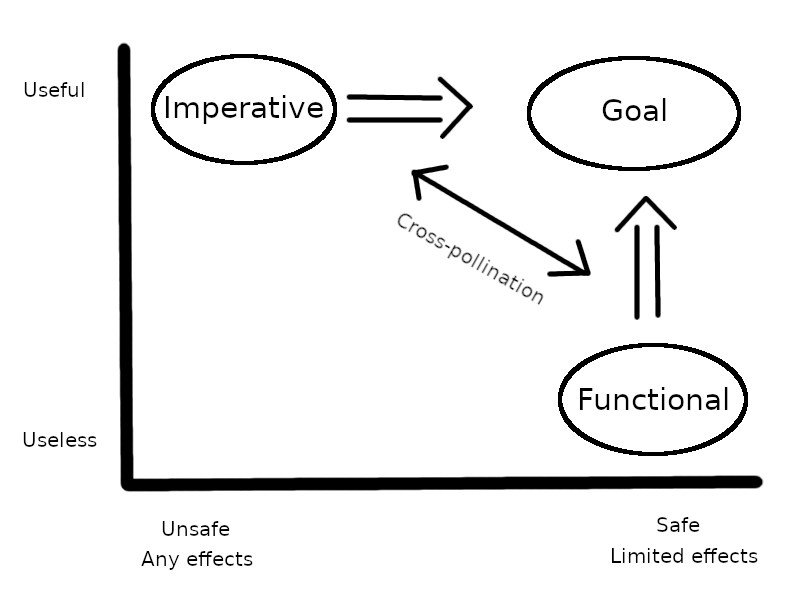
\includegraphics[scale=1.3]{useless}
\end{center}

He talks about how both paradigms want to be safe, expressive and useful, but
they take two different approaches. Although they take two different
approaches, they borrorw a lot of ideas from eachother.

I personally quite like Rust. It's a low level language, but with a lot of
cheap abstractions. In the laziness examples I used Rust (section
\ref{laziness}). It was quite clear in those examples that there was more going
on then what I was explaining. All this extra was technical details the Rust
compiler requires, but Rust also provides a vocabulary for more abstract ideas.
Rust takes a middle way, it tries to have expressiveness and abstraction
without losing out on speed and technical details. This does make Rust quite a
complicated and large language---it's not as elegant as C or Haskell. Haskell
is relatively simple and elegant, and so is C. C is very nice if you have to
perform relatively simple tasks where speed and optimisation is important,
while Haskell is very nice when you have to write very complicated systems
where performance isn't an issue. Rust provides a vocabulary to solve big and
complicated where performance is an issue. It tries to fill the same gap C++
does, but C++ has been hacked on and added to for what feels like centuries. It
is becoming a convoluted monster. Rust starts with a clean slate and new ideas
and experience from C++.

\subsubsection{Meta programming}\label{metaprogramming}

There is another paradigm I want to have a quick look at. This is \emph{meta
programming}. Most programmers are probably familiar with meta programming.
It's when you write code that generates code. Most languages have macro's and
something along the lines of C++'s template system. These are all forms of meta
programming, but there are languages that have \emph{only} meta programming.
Meta programming allows for a lot of abstraction. You can easily abstract
repetative code.

Probably the biggest meta programming language (family) is Lisp. Lisp is very
simple, just like the lambda calculus. It only has lists. Your program is
entierly made up of lists. Lists can be evaluated. The resulting language has
some similarities to lambda calculus and functional programming. Namely, in
lambda calculus everything is a function that can be evaluated, while in Lisp,
everything is a list that can be evaluated.

\section{A practical example of functional programming}

Section \ref{comparison} compares functional programming with other paradigms.
I thought it would be interesting to do a practical example. In section
\ref{metaprogramming}, I talked about the Lisp programming language family, in
particular Scheme. It isn't all to hard to implement a Lisp-like language, but
implementing a programming language is very conceptual. Programming languages
have many abstract concepts that are more easily expressed in a
declarative/functional language like Haskell, rather than a
procedural/imperative language like C. This section is really a practical
continuation of section \ref{comparison}, so I recommend you read it before you
read this. This section tries to paint a picture of what is said in section
\ref{comparison}.

I sadly didn't have the time to completely finish the interpreters, but I have
written some code that already shows what I'm trying to get at. I'll go over
what an interpreter should do and how you would go about implementing that in C
and Haskell. I got pretty far with the C interpreter, though.

\subsection{How an interpreter works}

We first have to understand how an interpreter actually works before we start
writing one. An interpreter should perform a few steps.

\subsection{Lisp interpreter in C}

I can't just paste all the code in here, that would be stupid, so you can find
it in the accompanying code folder. You're not going to understand most of the
code, but that's the point. I'm trying to show that the semantics of code is
much more obvious in Haskell than in C.

\subsection{Lisp interpreter in Haskell}

\newpage
\section*{Afterword}

\newpage
\section*{Unreferenced resources}

\addcontentsline{toc}{section}{Afterword}
\addcontentsline{toc}{section}{Unreferenced resources}

\newpage
\printbibliography[heading=bibintoc, title={References}]

\end{document}
